\documentclass[10pt]{article}
\usepackage{preamble}

\def\FS{Formelsammlung}
\def\Fach{Felder, Wellen und Leitungen}
\title{\FS \\ \Fach}
\date{\today}
\def\Semester{Sommersemester 23}
\IfFileExists{info.tex}
{
    \input{info.tex}
}
{
    \author{\href{https://www.youtube.com/watch?v=yMR45cZbvDw}{Die Prinzen - Alles nur geklaut}}
    \def\MatNr{MATNR}
}

\begin{document}

\pagenumbering{gobble}
\begin{titlepage}
    \thispagestyle{empty}

    \begin{center}
        \includegraphics[width=0.7\textwidth]{OTHR_OTHR_Logo}\\
        \vspace*{\stretch{1}}
        \Huge
        \textsc{\MyTitle}\\
        \vspace*{\stretch{0.25}}
        \normalsize
        \Semester

        \vspace*{\stretch{2}}
        {\renewcommand{\arraystretch}{1.5}
            \begin{tabular}{l l}
                Name:            & \hspace{4cm}\MyAuthor \\
                Matrikelnummer:  & \hspace{4cm}\MatNr    \\
                Letzte Änderung: & \hspace{4cm}\MyDate   \\
                Lizenz:          & \hspace{4cm}GPLv3
            \end{tabular}
        }
        \vspace*{\stretch{1}}

    \end{center}
\end{titlepage}

\newpage


\tableofcontents\clearpage

\pagestyle{fancy}
\lhead{\MyAuthor}
\rhead{\Semester}
\cfoot{\vspace{-20pt}\thepage}
\pagenumbering{arabic}
% \setlength{\columnsep}{1pt}
\raggedcolumns


\begin{multicols*}{2}
    \section{Grundlagen}
\subsection{Einheiten}
% \begin{table}[H]
% 	\renewcommand{\arraystretch}{2.15}
% \begin{tabularx}{0.9\columnwidth}{lXl}

\subsection{Vektorrechnung}
\subsubsection{Betrag, Richtungswinkel, Normierung}
\textbf{Betrag}
\begin{align*}
	\vert \vec{r}  \vert & = r = \sqrt{r^2_x + r^2_y + r^2_z}
\end{align*}
\textbf{Richtungswinkel}
\begin{align*}
	\cos(\alpha) = \dfrac{a_x}{\vert \vec{a} \vert} \qquad \cos(\beta) = \dfrac{a_y}{\vert \vec{a} \vert} \qquad
	\cos(\gamma) = \dfrac{a_z}{\vert \vec{a} \vert}
\end{align*}
\textbf{Normierung, Einheitsvektor}
\begin{align*}
	\vec{e}_a =  \dfrac{\vec{a}}{\vert \vec{a} \vert}, \quad \vert \vec{e}_a \vert = 1
\end{align*}

\subsubsection{Skalarprodukt} (Schnittwinkel zweier Vektoren)
\begin{align*}
	\vec{a} \cdot \vec{b} & = |\vec{a}| \cdot |\vec{b}| \cdot cos(\varphi) \qquad \vec{a} \cdot \vec{b}  = 0\\
	cos(\varphi)          &  = \dfrac{\vec{a} \cdot \vec{b}}{|\vec{a}| \cdot |\vec{b}|} = \dfrac{a_x \cdot b_x + a_y \cdot b_y + a_z \cdot b_z}{|\vec{a}| \cdot |\vec{b}|}
\end{align*}

\subsubsection{Kreuzprodukt}

\begingroup
\renewcommand*{\arraystretch}{.95}
\begin{align*}
	A_{Para} & = \vert \vec{c} \vert = \vert \vec{a} \times \vec{b} \vert = \vert \vec{a} \vert \cdot \vert \vec{b} \vert \cdot \sin(\varphi)\\
	\vec{a}\times\vec{b} & =
	\begin{pmatrix}
		a_x \\
		a_y \\
		a_z
	\end{pmatrix}
	\times
	\begin{pmatrix}
		b_x \\
		b_y \\
		b_z
	\end{pmatrix} =
	\begin{pmatrix}
		a_yb_z-a_zb_y \\
		a_zb_x-a_xb_z \\
		a_xb_y-a_yb_x
	\end{pmatrix}
\end{align*}
\endgroup
Trick: Regel von Sarrus anwenden!

\subsection{Differentialoperatoren}
\textbf{Nabla-Operator}
\begin{align*}
    \nabla & = \vec{\nabla} = 
    \begin{psmallmatrix}
        \partial  / \partial x \\
        \partial  / \partial y \\
        \partial  / \partial z
    \end{psmallmatrix}
\end{align*}

\textbf{Laplace-Operator}
\begin{align*}
    \varDelta  & = \vec{\nabla} \cdot \vec{\nabla} = \textrm{div (grad)} = 
    \dfrac{\partial ^2}{\partial x^2}+\dfrac{\partial ^2}{\partial y^2}+\dfrac{\partial ^2}{\partial z^2}
\end{align*}

\textbf{Divergenz} $\opdiv$: Vektorfeld $\rightarrow$ Skalar \qquad S.382\\
\small{Quelldichte, gibt für jeden Punkt im Raum an, ob Feldlinien entstehen oder verschwinden.}
\begin{align*}
    \boxed{\opdiv \vec{F} = \nabla \cdot \vec{F}}   =  \dfrac{\partial F_x}{\partial x} 
    + \dfrac{\partial F_y}{\partial y} + \dfrac{\partial F_z}{\partial z}\\ 
                                 \begin{cases}
    > 0 \quad\Rightarrow \textnormal{Quelle}  \\
    < 0 \quad\Rightarrow \textnormal{Senke} \\
    = 0 \quad\Rightarrow \textnormal{quellenfrei} 
\end{cases}                                      
\end{align*}
% Bsp: $\opdiv \vec{B} = 0$, da mag. Felder in sich geschlossen.\\

\textbf{Rotation} $\oprot$: Vektorfeld $\rightarrow$ Vektorfeld \qquad S.382\\ 
\small{Wirbeldichte, gibt für jeden Punkt im Raum Betrag und Richtung der Rotationsgeschwindigkeit an.}
\begin{align*}
\boxed{\oprot \vec{F} = \nabla \times \vec{F} } = 
\begin{pmatrix}
    \dfrac{\partial F_z}{\partial y} - \dfrac{\partial F_y}{\partial z} \\
    \dfrac{\partial F_x}{\partial z} - \dfrac{\partial F_z}{\partial x} \\
    \dfrac{\partial F_y}{\partial x} - \dfrac{\partial F_x}{\partial y}
\end{pmatrix} =
\begin{vmatrix}
    \vec{e}_x & \vec{e}_y & \vec{e}_z \\
    \dfrac{\partial}{\partial x} & \dfrac{\partial }{\partial x} & \dfrac{\partial }{\partial z} \\
    \vec{F}_x & \vec{F}_y & \vec{F}_z
\end{vmatrix}
\end{align*}\\
Vektorfeld skalar annotiert: $\vec{F} = \vec{F}(x;y;z) = F_x\vec{e}_x+F_y\vec{e}_y+F_z\vec{e}_z$\\
% Bsp: energieerhaltende (konservatives) Felder $ \rightarrow \oprot = 0$\\

\textbf{Gradient} $\opgrad$: Skalarfeld $\rightarrow$ Vektor/Gradientenfeld\\ 
\small{zeigt in Richtung steilster Anstieg von $\phi$}
\begin{align*}                                                                                          
    \boxed{\opgrad \phi = \nabla \cdot \phi }=  
    % \hspace{4.5ex}
    \begin{psmallmatrix}
        \partial \phi / \partial x \\
        \partial \phi / \partial y \\
        \partial \phi / \partial z
        % \dfrac{\partial G}{\partial x}\\
        % \dfrac{\partial G}{\partial y}\\
        % \dfrac{\partial G}{\partial z}
    \end{psmallmatrix}
    = \dfrac{\partial \phi}{\partial x} \vec{e}_x + \dfrac{\partial \phi}{\partial y} \vec{e}_y + 
    \dfrac{\partial \phi}{\partial z} \vec{e}_z  
\end{align*}

\subsubsection{Rechenregeln}
$\phi, \psi$: Skalarfelder \qquad $\vec{A}, \vec{B}$: Vektorfelder
\begin{align*}
     & \nabla \cdot (\vec{A} \times \vec{B}) & = & \qquad (\nabla \times \vec{A})\cdot\vec{B} - (\nabla\times\vec{B})\cdot\vec{A} \\
     & \nabla \cdot (\phi \cdot \psi)        & = & \qquad \phi (\nabla \psi) + \psi( \nabla \phi)                                  \\
     & \nabla \cdot (\phi \cdot \vec{A})           & = & \qquad \phi (\nabla \vec{A}) + \vec{A}(\nabla \phi)                             \\
     & \nabla \times (\phi \cdot \vec{A})          & = & \qquad \nabla \phi \times \vec{A} + \phi (\nabla \times \vec{A})                        
    %  & \oprot \opgrad f                      & = & \qquad 0 \Rightarrow\textnormal{Gradientenfeld Quellenfrei}                    \\
    %  & \opdiv \oprot \vec{f}                 & = & \qquad 0 \Rightarrow\textnormal{Wirbelfeld Quellenfrei}
\end{align*}

\subsubsection{Spezielle Vektorfelder}
quellenfreies Vektorfeld $\vec{F}$ $\rightarrow$ Vektorpotential $\vec{E}$
\begin{align*}
\opdiv \vec{F} = \boxed{\opdiv (\oprot \vec{E}) = 0} \quad \Leftrightarrow \quad  \vec{F} = \oprot \vec{E}
\end{align*}
wirbelfreies Vektorfeld $\vec{F}$ $\rightarrow$ Skalarpotential $\phi$
\begin{align*}
    \oprot \vec{F} = \boxed{\oprot (\opgrad \phi) = 0} \quad \Leftrightarrow \quad  \vec{F} = \opgrad \phi
\end{align*}
quellen- und wirbelfreies Vektorfeld $\vec{F}$:
\begin{align*}
    &\oprot \vec{F}  = 0 \quad \opdiv \vec{F} = 0\\
    &\opdiv (\opgrad \phi) = \varDelta \phi = 0 \quad \Leftrightarrow \quad  \vec{F} = \opgrad \phi\\
    &\oprot (\oprot \vec{F})  = \opgrad (\opdiv \vec{F}) - \varDelta \vec{F} 
\end{align*}

    \subsection{Logarithmische Maße/Pegel}
	Wichtig: Feldgrößen sind \textbf{Effektivwerte}!
        \begin{itemize} 
            \item \textbf{Dämpfungsmaß} $ a $ in Dezibel [dB] und Neper [Np]
            \begin{flalign*}
                1 \, \si{dB} & =  0,1151 \, \si{Np} & 1 \, \si{Np} & = 8,686 \, \si{dB} & \\  
                a \,[\si{dB}]  & = 20 \cdot \log_{} \dfrac{F_1}{F_2} & a \,[\si{dB}]  & = 10 \cdot \log_{}  \frac{P_1}{P_2}& \\
                \frac{F_1}{F_2} & =  10^{\frac{a[\si{dB}]}{20\si{dB}}} & \frac{P_1}{P_2}   & =   10^{\frac{a[\si{dB}]}{10\si{dB}}} &\\
                a \,[\si{Np}]  & = \ln \dfrac{F_1}{F_2} & a \,[\si{Np}]  & = \dfrac{1}{2} \cdot \ln \dfrac{P_1}{P_2} & \\
                \frac{F_1}{F_2} & =  e^{a[\si{Np}]}                   & \frac{P_1}{P_2}   & = e^{2a[\si{Np}]} &
	            \end{flalign*}
        	\item \textbf{absolute Pegel} $ L $ mit Bezugsgrößen $ P_0, F_0 $
			\begin{flalign*}
				L \,[\si{dB}]  & = 20 \cdot \log_{} \dfrac{F_1}{F_0} & L \,[\si{dB}]  & = 10 \cdot \log_{}  \frac{P_1}{P_0}& \\
				\frac{F_1}{F_0} & =  10^{\frac{L[\si{dB}]}{20\si{dB}}} & \frac{P_1}{P_0}   & =   10^{\frac{L[\si{dB}]}{10\si{dB}}} &
			\end{flalign*}
            \renewcommand\arraystretch{1.4}
			\begin{tabularx}{0.8\columnwidth}{l|X|X}
			\hline
			Einheit & Bezugswert & Formelzeichen\\
			\hline
			dBm, dB(mW) & $ P_0 = 1mW $ & $ L_{\texttt{P/mW}}$ \\
			dBW, dB(W) & $ P_0 = 1W $ & $ L_{\texttt{P/W}}$ \\
			\hline
			\end{tabularx}
			
        \item \textbf{relativer Pegel / Maß}\\
        Maß = Differenz zweier (Leistungs)pegel bei\\ gleichem Bezugswert $ P_0 $
        \begin{equation*}
        	\Delta L = L_2 - L_1 = 10 \cdot \log \left( \frac{P_2}{P_1}\right)  \si{dB}
        \end{equation*}
        \end{itemize}

\subsubsection{Rechnen mit Pegeln / Logarithmen}
Rechenregeln für Logarithmen (10er-Basis): \quad $ x,y,a > 0 $
\begin{flalign*}
	\log (x\cdot y) &= \log (x) - \log (y) & \log (\tfrac{x}{y}) & = \log (x) - \log (y) &\\
	\log (x^a) &= a\cdot \log(x)  & \log \sqrt[a]{x} & = \frac{1}{a} \cdot \log (x) &\\
   \mathtt{Pegel} &= 10 \cdot \log(\mathtt{Faktor}) & \mathtt{Faktor}& = 10 ^{\tfrac{\mathtt{Pegel}}{10}}
\end{flalign*}

\subsection{Rechnen mit Wurzeln}
$a$: Radikant \qquad $n$: Wurzelexponent\\
Merke: $\sqrt[n]{a \pm b} \neq \sqrt[n]{a} \pm \sqrt[n]{b}$ \qquad $ x = \sqrt[n]{a} = a^{\frac{1}{n}} $
\begin{flalign*}
&\sqrt[n]{a^m}=\left(a^m\right)^{\frac{1}{n}}=\left(a^{\frac{1}{n}}\right)^m=a^{\frac{m}{n}}=(\sqrt[n]{a})^m\\
&\sqrt[m]{\sqrt[n]{a}}=\sqrt[m]{a^{\frac{1}{n}}}=\left(a^{\frac{1}{n}}\right)^{\frac{1}{m}}=a^{\frac{1}{m \cdot n}}=\sqrt[m \cdot n]{a}\\
&\sqrt[n]{a} \cdot \sqrt[n]{b}=\left(a^{\frac{1}{n}}\right) \cdot\left(b^{\frac{1}{n}}\right)=(a b)^{\frac{1}{n}}=\sqrt[n]{a b}\\
&\frac{\sqrt[n]{a}}{\sqrt[n]{b}}=\frac{a^{\frac{1}{n}}}{b^{\frac{1}{n}}}=\left(\frac{a}{b}\right)^{\frac{1}{n}}=\sqrt[n]{\frac{a}{b}} \quad(b>0)
\end{flalign*}

\subsection{Rechnen mit Potenzen}
$a$: Basis \qquad $m,n$: Exponent
\begin{flalign*}
	&a^m \cdot a^n=a^{m+n} & \frac{a^m}{a^n}&=a^{m-n} \quad(a \neq 0)&\\
	&\left(a^m\right)^n=\left(a^n\right)^m=a^{m \cdot n}& a^n \cdot b^n&=(a \cdot b)^n&\\
	& \frac{a^n}{b^n}=\left(\frac{a}{b}\right)^n \quad(b \neq 0)& a^b &= e^{b \cdot \ln a}&\\
	&a^0 =1 & a^{-n} &= \frac{1}{a^n}&
\end{flalign*}


\subsection{Integralsätze}
\begin{align*}
    \int_{a}^b \opgrad F \cdot d \vec{s}     & = F(b) - F(a)                                  \\
    \iiint_V \opdiv \vec{A} \cdot dV         & = \oiint_{ \partial V} \vec{A} \cdot d \vec{a} \\
    \iint_{A} \oprot \vec{A} \cdot d \vec{a} & = \oint_{ \partial A} \vec{A} \cdot d \vec{r}
\end{align*}

\subsubsection{Rechenregeln}
\begin{align*}
    \int x + y \, dx &= \frac{x^2}{2} + xy
\end{align*}


\subsection{Koordinatensysteme}

\subsubsection{Umrechnungstabelle}
\begin{tabularx}{0.45\textwidth}{>{\hsize=.46\hsize}X|>{\hsize=.27\hsize}X|>{\hsize=.27\hsize}X}
    Kart.                                                                                & Zyl.             & Kug.                            \\
    \specialrule{1.5pt}{0pt}{0pt}
    $x$                                                                                  & $r \cos \varphi$ & $r \sin \vartheta \cos \varphi$ \\
    \hline
    $y$                                                                                  & $r \sin \varphi$ & $r \sin \vartheta \sin \varphi$ \\
    \hline
    $z$                                                                                  & $z$              & $r \cos \vartheta$              \\
    \specialrule{1.5pt}{0pt}{0pt}
    $\sqrt{x^{2}+y^{2}}$                                                                 & $r$              &                                 \\
    \hline
    $\arctan \frac{y}{x}$                                                                & $\varphi$        &                                 \\
    \hline
    $z$                                                                                  & $z$              &                                 \\
    \hline
    $d x \cos \varphi+d y \sin \varphi$                                                  & $dr$             &                                 \\
    \hline
    $d y \cos \varphi-d x \sin \varphi$                                                  & $r d\varphi$     &                                 \\
    \hline
    $dz$                                                                                 & $dz$             &                                 \\
    \specialrule{1.5pt}{0pt}{0pt}
    $\sqrt{x^{2}+y^{2}+z^{2}}$                                                           &                  & $r$                             \\
    \hline
    $\arctan \frac{y}{x}$                                                                &                  & $\varphi$                       \\
    \hline
    $\arctan \frac{\sqrt{x^{2}+y^{2}}}{z}$                                               &                  & $\vartheta$                     \\
    \hline
    $d x \sin \vartheta \cos \varphi+d y \sin \vartheta \sin \varphi+d z \cos \vartheta$ &                  & $dr$                            \\
    \hline
    $d y \cos \varphi-d x \sin \varphi$                                                  &                  & $r \sin \vartheta d \varphi$    \\
    \hline
    $d x \cos \vartheta \cos \varphi+d y \cos \vartheta \sin \varphi-d z \sin \vartheta$ &                  & $r d \vartheta$                 \\
\end{tabularx}

\subsubsection{Schema KOS Kugel/Zylinder}
\tdplotsetmaincoords{70}{110}

%Macros  
\pgfmathsetmacro{\rvec}{6}  
\pgfmathsetmacro{\thetavec}{40}  
\pgfmathsetmacro{\phivec}{45}

\pgfmathsetmacro{\dphivec}{20}  
\pgfmathsetmacro{\dthetavec}{20}  
\pgfmathsetmacro{\drvec}{1.5}

%Layers  
\pgfdeclarelayer{background} 
\pgfdeclarelayer{foreground}

\pgfsetlayers{background, main, foreground}

%Kugelkoordinaten
\scalebox{0.55}
{

	\begin{tikzpicture}[tdplot_main_coords]
	%Coordinates  
	\coordinate (O) at (0,0,0);  
	\tdplotsetcoord{A}{\rvec}{\thetavec}{\phivec}  
	\tdplotsetcoord{B}{\rvec}{\thetavec + \dthetavec}{\phivec}         
	\tdplotsetcoord{C}{\rvec}{\thetavec + \dthetavec}{\phivec + \dphivec}  
	\tdplotsetcoord{D}{\rvec}{\thetavec}{\phivec + \dphivec}  
	\tdplotsetcoord{E}{\rvec + \drvec}{\thetavec}{\phivec}  
	\tdplotsetcoord{F}{\rvec + \drvec}{\thetavec + \dthetavec}{\phivec}  
	\tdplotsetcoord{F'}{\rvec + \drvec}{90}{\phivec}  \tdplotsetcoord{G}{\rvec + \drvec}{\thetavec + \dthetavec}{\phivec + \dphivec}  
	\tdplotsetcoord{G'}{\rvec + \drvec}{90}{\phivec + \dphivec} 
	\tdplotsetcoord{H}{\rvec + \drvec}{\thetavec}{\phivec + \dphivec} 
	
	%Axis  
	\begin{pgfonlayer}{background}  
		\draw[thick,-latex] (0,0,0) -- (7,0,0) node[pos=1.1]{$x$};        
		\draw[thick,-latex] (0,0,0) -- (0,7,0) node[pos=1.05]{$y$};         
		\draw[thick,-latex] (0,0,0) -- (0,0,6) node[pos=1.05]{$z$};                   
	\end{pgfonlayer}
	
	%Help Lines  
	\begin{pgfonlayer}{background}  
		%Up     
		\draw[thick, blue] (O) -- (A) node[pos=0.6, above left, blue] {$r$};    
		\draw (O) -- (B);   
		\draw (O) -- (C);   
		\draw[dashed] (O) -- (D);   
		%Down   
		\draw (O) -- (F');  
		\draw (O) -- (G');  
	\end{pgfonlayer}  
	\begin{pgfonlayer}{foreground}  
		%%Help Curves   
		\tdplotsetthetaplanecoords{\phivec}     
		\tdplotdrawarc[tdplot_rotated_coords]{(O)}{\rvec}{\thetavec+\dthetavec}{90}{}{}
		%
		\tdplotdrawarc[tdplot_rotated_coords]{(O)}{\rvec+\drvec}{\thetavec+\dthetavec}{90}{}{}
		%
		\tdplotsetthetaplanecoords{\phivec+\dphivec}    
		\tdplotdrawarc[tdplot_rotated_coords, dashed]{(O)}{\rvec}{\thetavec+\dthetavec}{90}{}{}     
		\tdplotdrawarc[tdplot_rotated_coords]{(O)}{\rvec+\drvec}{\thetavec+\dthetavec}{90}{}{}
		%   
		\tdplotdrawarc[tdplot_main_coords]{(O)}{\rvec}{\phivec}{\phivec+\dphivec}{}{}
		%    
		\tdplotdrawarc[tdplot_main_coords]{(O)}{\rvec+\drvec}{\phivec}{\phivec+\dphivec}{below, rotate=13}{$r\sin\vartheta\,\mathrm{d}\varphi$} 
	\end{pgfonlayer}
	
	
	%Angles  
	\begin{pgfonlayer}{foreground}  
		%Phi, dPhi  
		\tdplotdrawarc[-stealth]{(O)}{0.9}{0}{\phivec}{anchor=north}{$\varphi$}    
		\tdplotdrawarc[-stealth]{(O)}{1.5}{\phivec}{\phivec + \dphivec}{}{}     
		\node at (1.4,1.9,0) {$\mathrm{d}\varphi$};        
		\tdplotsetthetaplanecoords{\phivec}     
		%Theta, dTheta          
		\tdplotdrawarc[tdplot_rotated_coords,-stealth]{(0,0,0)}{1.2}{0}{\thetavec}{}{}      
		\node at (0,0.3,1.3) {$\vartheta$};    
		\tdplotdrawarc[tdplot_rotated_coords,-stealth]{(0,0,0)}{2.5}{\thetavec}{\thetavec + \dthetavec}{anchor=south west}{$\mathrm{d}\vartheta$}  
	\end{pgfonlayer}
	
	%Differential Volume
	
	%%Lines  
	\begin{pgfonlayer}{foreground}  
		\draw[thick] (A) -- (E) node[midway, above left]{$\mathrm{d}r$};    
		\draw[thick] (B) -- (F);    
		\draw[thick] (C) -- (G);      
	\end{pgfonlayer}   
	\begin{pgfonlayer}{background}
		\draw[dashed, thick] (D) -- (H);  
	\end{pgfonlayer}
	
	%%Curved 
	\begin{pgfonlayer}{background}      
		\tdplotsetrotatedcoords{55}{-50.4313}{-6.4086}  
		\tdplotdrawarc[dashed, tdplot_rotated_coords, thick]{(O)}{\rvec}{0}{12.8173}{}{}
		%   
		\tdplotsetthetaplanecoords{\phivec + \dphivec}  
		\tdplotdrawarc[dashed, tdplot_rotated_coords, thick]{(O)}{\rvec}{\thetavec}{\dthetavec + \thetavec}{}{}  
	\end{pgfonlayer} 
	\begin{pgfonlayer}{foreground}     
		\tdplotsetthetaplanecoords{\phivec}     
		\tdplotdrawarc[tdplot_rotated_coords, thick]{(O)}{\rvec}{\thetavec}{\dthetavec + \thetavec}{}{}     
		\tdplotdrawarc[tdplot_rotated_coords, thick]{(O)}{\rvec + \drvec}{\thetavec}{\dthetavec + \thetavec}{}{}
		%   
		\tdplotsetthetaplanecoords{\phivec + \dphivec}  
		\tdplotdrawarc[tdplot_rotated_coords, thick]{(O)}{\rvec + \drvec}{\thetavec}{\dthetavec + \thetavec}{above right}{$r\mathrm{d}\vartheta$}  
		%   
		\tdplotsetrotatedcoords{55}{-50.4313}{-6.4086}  
		\tdplotdrawarc[tdplot_rotated_coords, thick]{(O)}{\rvec + \drvec}{0}{12.8173}{}{}   
		%   
		\tdplotsetrotatedcoords{55}{-30.3813}{-8.6492}          
		\tdplotdrawarc[tdplot_rotated_coords, thick]{(O)}{\rvec}{0}{17.2983}{}{}    
		\tdplotdrawarc[tdplot_rotated_coords, thick]{(O)}{\rvec + \drvec}{0}{17.2983}{}{}  
	\end{pgfonlayer}
	
	%Fill Color 
	\begin{pgfonlayer}{main}    
		%Front  
		\fill[black!30, opacity=0.15] (E) to (A)  to[bend left=4] (B) to (F) to[bend right=4] cycle;   
		\fill[black!30, opacity=0.6] (E) to[bend left=4] (F)  to[bend left=2] (G) to[bend right=6.5] (H) to[bend right=4] cycle;   
		\fill[black!30, opacity=0.4] (F) to[bend left=2] (G) to[bend left=1.5] (C) to[bend right=2.5] (B) to[bend right=4] cycle;   
	\end{pgfonlayer}  
	\begin{pgfonlayer}{background}  
		%Back   
		\fill[black!20, opacity=0.5] (A) to[bend left=2] (D) to[bend left=6] (C) to[bend right=2.5] (B) to[bend right=4] cycle;     
		\fill[black!20, opacity=0.5] (A) to[bend left=2] (D) to (H) to[bend right=2.5] (E) to[bend right=4] cycle;  
		\fill[black!20, opacity=0.5] (D) to (H) to[bend left=6] (G) to[bend right=2] (C) to[bend right=6] cycle;  
	\end{pgfonlayer}
\end{tikzpicture}
}

%\Zylinderkoordinaten
\scalebox{0.55}
{
%Cylindrical Coordinate
\newcommand{\cylindricalcoordinate}[4]{%
	\coordinate (#4) at ({#1*cos(#2)},{#1*sin(#2)},{#3});%
	\coordinate (#4xy) at ({#1*cos(#2)},{#1*sin(#2)},0);%
}

%Axis Angles
\tdplotsetmaincoords{70}{110}

%Macros
\pgfmathsetmacro{\rvec}{5}
\pgfmathsetmacro{\phivec}{45}
\pgfmathsetmacro{\zvec}{4}

\pgfmathsetmacro{\drvec}{1.5}
\pgfmathsetmacro{\dphivec}{20}
\pgfmathsetmacro{\dzvec}{1}

%Layers
\pgfdeclarelayer{background}
\pgfdeclarelayer{foreground}

\pgfsetlayers{background, main, foreground}

\begin{tikzpicture}[tdplot_main_coords]
	
	%Coordinates
	\coordinate (O) at (0,0,0);
	%%
	\cylindricalcoordinate{\rvec}{\phivec}{\zvec}{A}
	\cylindricalcoordinate{\rvec}{\phivec}{(\zvec+\dzvec)}{B}
	\cylindricalcoordinate{\rvec}{(\phivec+\dphivec)}{\zvec}{C}
	\cylindricalcoordinate{\rvec}{(\phivec+\dphivec)}{(\zvec+\dzvec)}{D}
	%%
	\cylindricalcoordinate{(\rvec+\drvec)}{\phivec}{\zvec}{A'}
	\cylindricalcoordinate{(\rvec+\drvec)}{\phivec}{(\zvec+\dzvec)}{B'}
	\cylindricalcoordinate{(\rvec+\drvec)}{(\phivec+\dphivec)}{\zvec}{C'}
	\cylindricalcoordinate{(\rvec+\drvec)}{(\phivec+\dphivec)}{(\zvec+\dzvec)}{D'}
	%%%Nodes
	%\node at (A) {A};
	%\node at (B) {B};
	%\node at (C) {C};
	%\node at (D) {D};
	%\node at (A') {A'};
	%\node at (B') {B'};
	%\node at (C') {C'};
	%\node at (D') {D'};
	
	%Axis
	\begin{pgfonlayer}{background}
		\draw[thick,-latex] (0,0,0) -- (6,0,0) node[pos=1.1]{$x$};
		\draw[thick,-latex] (0,0,0) -- (0,6,0) node[pos=1.05]{$y$};
		\draw[thick,-latex] (0,0,0) -- (0,0,7) node[pos=1.05]{$z$};
	\end{pgfonlayer}
	
	%Vectors
	\begin{pgfonlayer}{main}
		\draw[blue, thick] (O) -- (A);
		\draw[thick] (O) -- (Axy) node [pos=0.6, below left] {$r$};
		\draw (A) -- ($(A)-(Axy)$) node [left] {$z$};
		\draw (B) -- ($(A)-(Axy)+(0,0,\dzvec)$) node [left] {$z+\mathrm{d}z$};
		\draw (D) -- ($(A)-(Axy)+(0,0,\dzvec)$);
	\end{pgfonlayer}
	\begin{pgfonlayer}{background}
		\draw[dashed] (C) -- ($(A)-(Axy)$) node [left] {$z$};
	\end{pgfonlayer}
	
	%Help Lines
	\begin{pgfonlayer}{background}
		\draw (A) -- (Axy);
		\draw (A') -- (A'xy);
		\draw[thick] (Axy) -- (A'xy) node [pos=0.6, below left] {$\mathrm{d}r$};
		%
		\draw (O) -- (D'xy);
		\draw[dashed] (C) -- (Dxy);	
		\draw (C') -- (C'xy);
		%%Arcs
		\tdplotdrawarc{(0,0,0)}{\rvec}{\phivec}{\phivec+\dphivec}{}{}
		\tdplotdrawarc{(0,0,0)}{\rvec+\drvec}{\phivec}{\phivec+\dphivec}{}{}
	\end{pgfonlayer}
	
	%Angles
	\begin{pgfonlayer}{foreground}
		%Phi, dPhi
		\tdplotdrawarc[-stealth]{(O)}{0.9}{0}{\phivec}{anchor=north}{$\phi$}
		\tdplotdrawarc[-stealth]{(O)}{1.5}{\phivec}{\phivec + \dphivec}{}{}
		\node at (1.4,1.9,0) {$\mathrm{d}\varphi$};	
	\end{pgfonlayer}
	
	%Differential Volume
	
	%%Lines
	\begin{pgfonlayer}{foreground}
		\draw[thick] (A) -- (B) -- (B') -- (A') -- cycle node [midway, below] {$\mathrm{d}r$};
		\draw[thick] (D) -- (D') -- (C') node [midway, right] {$\mathrm{d}z$};
	\end{pgfonlayer}
	\begin{pgfonlayer}{background}
		\draw[thick, dashed] (C') -- (C) -- (D);
	\end{pgfonlayer}
	
	%%Curved
	\begin{pgfonlayer}{background}
		\tdplotdrawarc[thick, dashed]{(0,0,\zvec)}{\rvec} {\phivec}{\phivec+\dphivec}{}{}
	\end{pgfonlayer}
	\begin{pgfonlayer}{foreground}
		\tdplotdrawarc[thick]{(0,0,\zvec+\dzvec)}{\rvec} {\phivec}{\phivec+\dphivec}{}{}
		\node at (2.4,3.4,\zvec+\dzvec) {$r\mathrm{d}\varphi$};
		\tdplotdrawarc[thick]{(0,0,\zvec+\dzvec)}{\rvec+\drvec} {\phivec}{\phivec+\dphivec}{}{}
		\tdplotdrawarc[thick]{(0,0,\zvec)}{\rvec+\drvec} {\phivec}{\phivec+\dphivec}{}{}
	\end{pgfonlayer}
	
	%%Fill Color
	\begin{pgfonlayer}{main}
		%Front
		\fill[black!10, opacity=0.15] (B) to (B') to[bend right=4] (D') to (D) to[bend left=4] cycle;
		\fill[black!10, opacity=0.6] (B') to[bend right=4] (D') to (C') to[bend left=4] (A') to cycle;
		\fill[black!10, opacity=0.4] (B) to (B')  to (A') to (A) to cycle;
	\end{pgfonlayer}
	\begin{pgfonlayer}{background}
		%Back
		\fill[black!20, opacity=0.5] (D) to (D') to (C') to (C) to cycle;
		\fill[black!20, opacity=0.5] (B) to[bend right=4] (D) to (C) to[bend left=4] (A) to cycle;
		\fill[black!20, opacity=0.5] (A) to (A') to[bend right=4] (C') to (C) to[bend left=4] cycle;
	\end{pgfonlayer}
	
	
\end{tikzpicture}

}

\end{multicols*}

% newpage
\subsubsection{Kartesische Koordinaten}
\footnotesize{
\begin{flalign*}
	&\text{Variablen:}\quad x,y,z \qquad \qquad \text{Einheitsvektoren:}\quad \vec{e}_x, \vec{e}_y,\vec{e}_z \qquad \qquad
	\text{Rechtssystem:}\quad \vec{e}_x \times \vec{e}_y=\vec{e}_z &&&\\
	&\text{Linienelemente:} \quad  ds=\sqrt{d x^{2}+d y^{2}+d z^{2}} = dx \cdot \vec{e}_x + dy \cdot \vec{e}_y + dz \cdot \vec{e}_z \\
	&\text{Volumenelemente:} \quad  dV = dx \, dy \, dz &&&\\
	&\text{Flächenelemente:} \quad  dA_{xy}= dx \, dy \, \vec{e}_z \quad dA_{yz} = dy \, dz \, \vec{e}_x \quad dA_{xz} = dx \, dz \, \vec{e}_y
	&&&\\
	&\text{Skalarfeld:}\quad \phi = \phi(x;y;z) \qquad \text{Vektorfeld:} \quad \boxed{\vec{F} = \vec{F}(x;y;z) = F_x\vec{e}_x+F_y\vec{e}_y+F_z\vec{e}_z} &&&\\
	&\text{\textbf{Gradient}:}\quad \opgrad \phi \equiv \nabla \phi=\frac{\partial \phi}{\partial x} \vec{e}_x+\frac{\partial \phi}{\partial y} \vec{e}_y+\frac{\partial \phi}{\partial z} \vec{e}_z
	\qquad\qquad \text{\textbf{Divergenz}:}
	\quad \opdiv \vec{D} \equiv \nabla \vec{D}=\frac{\partial D_{x}}{\partial x}+\frac{\partial D_{y}}{\partial y}+\frac{\partial D_{z}}{\partial z} 
	&&&\\
	&\text{\textbf{Rotation}:} \quad                   \operatorname{rot} \vec{E} \equiv \nabla \times \vec{E} =
	\left[\frac{\partial E_z}{\partial y}-\frac{\partial E_y}{\partial z}\right] \vec{e}_x+\left[\frac{\partial E_x}{\partial z}-\frac{\partial E_z}{\partial x}\right] \vec{e}_y+\left[\frac{\partial E_y}{\partial x}-\frac{\partial E_x}{\partial y}\right] \vec{e}_z&&&\\
	&\text{\textbf{La-Place}}: \quad \Delta \equiv \nabla\cdot\nabla =\frac{\partial^{2}}{\partial x^{2}}+\frac{\partial^{2}}{\partial y^{2}}+\frac{\partial^{2}}{\partial z^{2}} \qquad                   
	\Delta \vec{E} = \opgrad \opdiv \vec{E}-\operatorname{rot} \operatorname{rot} \vec{E} = \Delta E_x \vec{e}_x+\Delta E_y \vec{e}_y+\Delta E_z \vec{e}_z \\
	&\Delta \vec{E} = \left[\frac{\partial^{2} E_x}{\partial x^{2}}+\frac{\partial^{2} E_x}{\partial y^{2}}+\frac{\partial^{2} E_x}{\partial z^{2}}\right] \vec{e}_x+\left[\frac{\partial^{2} E_y}{\partial x^{2}}+\frac{\partial^{2} E_y}{\partial y^{2}}+\frac{\partial^{2} E_y}{\partial z^{2}}\right] \vec{e}_y+ \left[\frac{\partial^{2} E_z}{\partial x^{2}}+\frac{\partial^{2} E_z}{\partial y^{2}}+\frac{\partial^{2} E_z}{\partial z^{2}}\right] \vec{e}_z     
	&&&\\
\end{flalign*}
}

\subsubsection{Zylinderkoordinaten}
Polarkoordinaten siehe S.386, Papula S.387, 
\begin{flalign*}
	&\text{Variablen:}\quad r,\varphi,z \qquad \qquad \text{Einheitsvektoren:}\quad \vec{e}_r, \vec{e}_\varphi,\vec{e}_z \qquad \qquad
	\text{Rechtssystem:}\quad \vec{e}_r \times \vec{e}_\varphi=\vec{e}_z &&&\\
	&\text{Linienelemente:} \quad  ds=\sqrt{d r^{2}+\mathbf{r} d \varphi^{2}+d z^{2}} = dr \cdot \vec{e}_r + \mathbf{r} \, d\varphi \cdot \vec{e}_\varphi + dz \cdot \vec{e}_z\\ &\text{Volumenelemente:} \quad  dV = \mathbf{r} \, dr \, d\varphi \, dz &&&\\
	&\text{Flächenelemente:} \quad  dA_{r\varphi} = \mathbf{r} \, dr \, d\varphi \, \vec{e}_z \quad dA_{rz} = dr \, dz \, \vec{e}_\varphi \quad dA_{\varphi z} = \mathbf{r} \, d\varphi \, dz \, \vec{e}_r
	&&&\\
	&\text{Skalarfeld:}\quad \phi = \phi(x;\varphi;z) \qquad \text{Vektorfeld:} \quad \boxed{\vec{F} = \vec{F}(r;\varphi;z) = F_r\vec{e}_r+F_\varphi\vec{e}_\varphi+F_z\vec{e}_z} &&&\\
	&\text{\textbf{Gradient}:}\quad \opgrad \phi \equiv \nabla \phi= \frac{\partial \phi}{\partial r} \vec{e}_r
	+\frac{1}{r} \frac{\partial \phi}{\partial \varphi} \vec{e}_\varphi
	+\frac{\partial \phi}{\partial z} \vec{e}_z &&&\\
	&\text{\textbf{Divergenz}:}
      \quad \opdiv \vec{D} \equiv \nabla \vec{D}=\frac{1}{r}\cdot\frac{\partial}{\partial r}\left(r\cdot\vec{D}_{r}\right)
		+\frac{1}{r}\cdot\frac{\partial \vec{D}_{\varphi}}{\partial \varphi}
		+\frac{\partial \vec{D}_{z}}{\partial z}
	&&&\\
	&\text{\textbf{Rotation}:}                   \quad \operatorname{rot} \vec{E} \equiv \nabla \times \vec{E}=
	\left[\frac{1}{r}\cdot\frac{\partial E_z}{\partial \varphi}-\frac{\partial E_\varphi}{\partial z}\right] \vec{e}_r
	+\left[\frac{\partial E_r}{\partial z}-\frac{\partial E_z}{\partial r}\right] \vec{e}_\varphi
	+\frac{1}{r}\left[\frac{\partial}{\partial r}\left(r\cdot E_\varphi\right)-\frac{\partial E_r}{\partial \varphi}\right] \vec{e}_z&&&\\
	&\text{\textbf{La-Place}}: \Delta\phi
	= \frac{1}{r}\cdot\frac{\partial }{\partial r}\left(r\cdot\frac{\partial\phi}{\partial r}\right)
	+ \frac{1}{r^2}\cdot\frac{\partial^2 \phi}{\partial \varphi^2}
	+ \frac{\partial^2 \phi}{\partial z^2} \qquad                   
	\Delta \vec{E} = \opgrad \opdiv \vec{E}-\operatorname{rot} \operatorname{rot} \vec{E} = \Delta E_r \vec{e}_r+\Delta E_\varphi \vec{e}_\varphi+\Delta E_z \vec{e}_z \\
	& \Delta \vec{E} =  \left[\Delta E_r-\frac{2}{r^{2}} \frac{\partial E_\varphi}{\partial \varphi}-\frac{E_r}{r^{2}}\right] \vec{e}_r
	+\left[\Delta E_\varphi+\frac{2}{r^{2}} \frac{\partial E_r}{\partial \varphi}-\frac{E_\varphi}{r^{2}}\right] \vec{e}_\varphi+\left[\Delta E_z\right] \vec{e}_z 
	&&&\\
\end{flalign*}

\subsubsection{Kugelkoordinaten}
\begin{flalign*}
	&\text{Variablen:}\quad r,\vartheta,\varphi \qquad \qquad \text{Einheitsvektoren:}\quad \vec{e}_r, \vec{e}_\vartheta,\vec{e}_\varphi \qquad \qquad
	\text{Rechtssystem:}\quad \vec{e}_r \times \vec{e}_\vartheta=\vec{e}_\varphi &&&\\
	&\text{Linienelemente:} \quad  ds=\sqrt{d r^{2}+ \mathbf{r^2} \sin^2 \vartheta \, d \varphi^{2}+\mathbf{r^2} d \vartheta^{2}} = dr \cdot \vec{e}_r + r \, d\vartheta \cdot \vec{e}_\vartheta + r \, \sin \varphi \,  d\varphi \cdot \vec{e}_\varphi \\
	&\text{Volumenelemente:} \quad  dV = \mathbf{r^2} \, \sin \vartheta \, dr \, d\vartheta \, d\varphi &&&\\
	&\text{Flächenelemente:} \quad  dA_{r\vartheta} = \mathbf{r}\, dr \, d\vartheta \, \vec{e}_\varphi \quad dA_{r\varphi} = \mathbf{r}\, \sin \, \vartheta \, dr \, d\varphi \, \vec{e}_\vartheta \quad dA_{\vartheta \varphi} = \mathbf{r^2} \, \sin \vartheta \, d\vartheta \, d\varphi \, \vec{e}_r
	&&&\\
	&\text{Skalarfeld:}\quad \phi = \phi(r;\vartheta;\varphi) \qquad \text{Vektorfeld:} \quad \boxed{\vec{F} = \vec{F}(r;\vartheta;\varphi) = F_r\vec{e}_r+F_\vartheta\vec{e}_\vartheta+F_\varphi\vec{e}_\varphi} &&&\\
	&\text{\textbf{Gradient}:}\quad                   \quad \opgrad \phi \equiv \nabla \phi=\frac{\partial \phi}{\partial r} \vec{e}_r+\frac{1}{r} \frac{\partial \phi}{\partial \vartheta} \vec{e}_\vartheta+\frac{1}{r \sin \vartheta} \frac{\partial \phi}{\partial \varphi} \vec{e}_\varphi &&&\\
	&\text{\textbf{Divergenz}:}
	                  \quad \opdiv \vec{D} \equiv \nabla \vec{D}=\frac{1}{r^{2}} \frac{\partial\left(r^{2} D_{r}\right)}{\partial r}+\frac{1}{r \sin \vartheta} \frac{\partial\left(\sin \vartheta \cdot D_{\vartheta}\right)}{\partial \vartheta}+\frac{1}{r \sin \vartheta} \frac{\partial D_{\varphi}}{\partial \varphi}
	&&&\\
	&\text{\textbf{Rotation}:} \quad                \operatorname{rot} \vec{E} = \frac{1}{r \sin \vartheta}\left[\frac{\partial\left(\sin \vartheta \cdot E_\varphi\right)}{\partial \vartheta}-\frac{\partial E_\vartheta}{\partial \varphi}\right] \vec{e}_r                                                                           
	+                           \frac{1}{r}\left[\frac{1}{\sin \vartheta} \frac{\partial E_r}{\partial \varphi}-\frac{\partial r E_\varphi}{\partial r}\right] \vec{e}_\vartheta+\frac{1}{r}\left[\frac{\partial\left(r E_\vartheta\right)}{\partial r}-\frac{\partial E_r}{\partial \vartheta}\right] \vec{e}_\varphi&&&\\
	&\text{\textbf{La-Place}}:                   \Delta\phi=\frac{1}{r^{2}}\left\{\frac{\partial}{\partial r}\left(r^2\cdot\frac{\partial\phi}{\partial r}\right)
	+\frac{1}{\sin\vartheta}\cdot\frac{\partial}{\partial\vartheta}\left(\sin\vartheta\cdot\frac{\partial\phi}{\partial\vartheta}\right)
	+\frac{1}{\sin^{2}\vartheta}\cdot\frac{\partial^{2}\phi}{\partial \varphi^{2}}\right\}\\
\end{flalign*}

Laplace Operator in Kugelkoordinaten, angewandt auf einen Vektor:
\footnotesize{
            \begin{multline*}
                  \Delta \vec{E}  =\left[\Delta E_r-\frac{2}{r^{2}} E_r-\frac{2}{r^{2} \sin \vartheta} \frac{\partial\left(\sin \vartheta \cdot E_\vartheta\right)}{\partial \vartheta}-\frac{2}{r^{2} \sin \vartheta} \frac{\partial E_\varphi}{\partial \varphi}\right] \vec{e}_r        \\
                  +\left[\Delta E_\vartheta-\frac{E_\vartheta}{r^{2} \sin ^{2} \vartheta}+\frac{2}{r^{2}} \frac{\partial E_r}{\partial \vartheta}-\frac{2 \cot \vartheta}{r^{2} \sin \vartheta} \frac{\partial E_\varphi}{\partial \varphi}\right] \vec{e}_\vartheta       \\
                  +\left[\Delta E_\varphi-\frac{E_\varphi}{r^{2} \sin ^{2} \vartheta}+\frac{2}{r^{2} \sin \vartheta} \frac{\partial E_r}{\partial \varphi}+\frac{2 \cot \vartheta}{r^{2} \sin \vartheta} \frac{\partial E_\vartheta}{\partial \varphi}\right] \vec{e}_\varphi
            \end{multline*}
      }

\section{Maxwell’schen Gleichungen}

\includegraphics[width=\columnwidth]{Figures/Integralsatz.png}

\textbf{Durchflutungssatz:}

\begin{tabularx}{\textwidth}{>{\hsize=.5\hsize}X>{\hsize=.5\hsize}X}
    Elektrischer Strom ist Ursache für magnetische Wirbelfeld & $\boxed{\int_c \vec{H} d \vec{s} = \Theta = I = \iint_A \vec{J} d \vec{A} = \frac{d\Phi_e}{dt}}$ \\
\end{tabularx}

\textbf{Induktionsgesetz:}

\begin{tabularx}{\textwidth}{>{\hsize=.5\hsize}X>{\hsize=.5\hsize}X}
    Ein sich zeitlich änderndes Magnetfeld erzeugt ein Elektrisches Wirbelfeld & $\boxed{\oint{\vec{E}d\vec{s}} = u_{ind} = -\frac{d}{dt}\iint{\vec{B}d\vec{A}} = -\frac{d\Phi_m}{dt}}$                          \\
                                                                               & $\boxed{rot{\vec{E}} = -\frac{\partial\vec{B}}{\partial t} = -\mu\cdot\frac{\partial\vec{H}}{\partial t} = -j\omega\mu\vec{H}}$
\end{tabularx}

\textbf{Differentielle ohmsche Gesetz:}

\begin{tabularx}{\textwidth}{>{\hsize=.5\hsize}X>{\hsize=.5\hsize}X}
    Bewegte elektrische Ladung erzeugt Magnetfeld & $\boxed{ rot \vec{H} = \vec{J} = \sigma \cdot \vec{E}} $
\end{tabularx}

Bei isotropen Stoffen sind $\varepsilon$ u. $\mu$ Skalare:
\[
    \varepsilon = \varepsilon_0 \cdot \varepsilon_r \qquad \mu = \mu_0 \cdot \mu_r
\]

\subsection{Integralsätze}
\begin{description}
    \setlength{\itemsep}{1pt}
    \item Fundamentalsatz der Analysis
    \item Gauß: Vektorfeld das aus Oberfläche von Volumen strömt muss aus Quelle in Volumen
    \item Stokes: innere Wirbel kompensieren $\rightarrow$ Rand betrachten
\end{description}
\begin{align*}
    \int_{a}^b \opgrad F \cdot d \vec{s}     & = F(b) - F(a)                                  \\
    \iiint_V \opdiv \vec{A} \cdot dV         & = \oiint_{ \partial V} \vec{A} \cdot d \vec{a} \\
    \iint_{A} \oprot \vec{A} \cdot d \vec{a} & = \oint_{ \partial A} \vec{A} \cdot d \vec{r}
\end{align*}



\begin{multicols*}{2}
    % \section{Maxwell’schen Gleichungen}

\includegraphics[width=\columnwidth]{Figures/Integralsatz.png}

\textbf{Durchflutungssatz:}

\begin{tabularx}{\textwidth}{>{\hsize=.5\hsize}X>{\hsize=.5\hsize}X}
    Elektrischer Strom ist Ursache für magnetische Wirbelfeld & $\boxed{\int_c \vec{H} d \vec{s} = \Theta = I = \iint_A \vec{J} d \vec{A} = \frac{d\Phi_e}{dt}}$ \\
\end{tabularx}

\textbf{Induktionsgesetz:}

\begin{tabularx}{\textwidth}{>{\hsize=.5\hsize}X>{\hsize=.5\hsize}X}
    Ein sich zeitlich änderndes Magnetfeld erzeugt ein Elektrisches Wirbelfeld & $\boxed{\oint{\vec{E}d\vec{s}} = u_{ind} = -\frac{d}{dt}\iint{\vec{B}d\vec{A}} = -\frac{d\Phi_m}{dt}}$                          \\
                                                                               & $\boxed{rot{\vec{E}} = -\frac{\partial\vec{B}}{\partial t} = -\mu\cdot\frac{\partial\vec{H}}{\partial t} = -j\omega\mu\vec{H}}$
\end{tabularx}

\textbf{Differentielle ohmsche Gesetz:}

\begin{tabularx}{\textwidth}{>{\hsize=.5\hsize}X>{\hsize=.5\hsize}X}
    Bewegte elektrische Ladung erzeugt Magnetfeld & $\boxed{ rot \vec{H} = \vec{J} = \sigma \cdot \vec{E}} $
\end{tabularx}

Bei isotropen Stoffen sind $\varepsilon$ u. $\mu$ Skalare:
\[
    \varepsilon = \varepsilon_0 \cdot \varepsilon_r \qquad \mu = \mu_0 \cdot \mu_r
\]

\subsection{Integralsätze}
\begin{description}
    \setlength{\itemsep}{1pt}
    \item Fundamentalsatz der Analysis
    \item Gauß: Vektorfeld das aus Oberfläche von Volumen strömt muss aus Quelle in Volumen
    \item Stokes: innere Wirbel kompensieren $\rightarrow$ Rand betrachten
\end{description}
\begin{align*}
    \int_{a}^b \opgrad F \cdot d \vec{s}     & = F(b) - F(a)                                  \\
    \iiint_V \opdiv \vec{A} \cdot dV         & = \oiint_{ \partial V} \vec{A} \cdot d \vec{a} \\
    \iint_{A} \oprot \vec{A} \cdot d \vec{a} & = \oint_{ \partial A} \vec{A} \cdot d \vec{r}
\end{align*}

    \section{Felder}
\subsection{Zusammenhänge}
Materialgleichungen
\begin{align*}
    \Aboxed{\vec{J}  = \kappa\vec{E}} & \Aboxed{\vec{B}  = \mu\vec{H}}    & \Aboxed{\vec{D}  = \varepsilon\vec{E}}\\
    \Aboxed{ rot \vec{H} = \vec{J} = \sigma \cdot \vec{E}} &
\end{align*}
\begin{align*}
    \Aboxed{&\oint_s{\vec{H} \, d\vec{s}} = \Theta = I = \iint_A \vec{J}  \, d\vec{A} = \frac{d\Phi_e}{dt}} \\
    \Aboxed{&\oint_s{\vec{E} \, d\vec{s}} = u_{ind} = -\frac{d}{dt}\iint{\vec{B} \, d\vec{A}} = -\frac{d\Phi_m}{dt}} \\
    \Aboxed{&rot{\vec{E}} = -\frac{\partial\vec{B}}{\partial t} = -\mu\cdot\frac{\partial\vec{H}}{\partial t} = -j\omega\mu\vec{H}}
\end{align*}

Feldunterscheidung
\begin{align*}
     & \vec{E}(x,y,z)                               & \widehat= & \quad\text{statisches Feld}  & \\
     & \vec{E}(x,y,z,t)                             & \widehat= & \quad\text{stationäres Feld} & \\
     & \vec{E}(x,y,z,t)\cdot cos(\omega t -\beta z) & \widehat= & \quad\text{Welle}            &
\end{align*}

\subsection{Elektrostatik}
\textbullet wirbelfreies Feld $\rightarrow$ Elektrische Ladungen sind Quellen des
Feldes
\begin{align*}
    \Aboxed{\opdiv \vec{D} & = \nabla \cdot \vec{D}  = \rho}\\
    \Aboxed{\oprot \vec{E} & = \nabla \times \vec{E} = 0} & \Aboxed{\oprot \opgrad E & = 0}\\
    \Aboxed{\vec{E} & = - \opgrad \varphi} \\
    Q &= \iiint_V \rho \, dV & U_{ab} = \int_{a}^{b} E \, ds
\end{align*}

\subsubsection{Potential Gleichung}
\[
    \opdiv \opgrad \varphi = - \dfrac{\rho}{\varepsilon}
\]

\textbf{$\qquad \Rightarrow$ Poisson-Gleichung}\\
mit $\rho = 0$ $\rightarrow$ \textbf{Laplace-Gleichung}
\begin{align*}
    \Delta \varphi + \underbrace{ \dfrac{\opgrad \varepsilon \cdot \opgrad \varphi}{\varepsilon}}_{= 0\texttt{, wenn homogen}}
     & = - \dfrac{\rho (x, y, z)}{\varepsilon} \\
    \frac{d^2 \varphi}{d x^2} + \frac{d^2 \varphi}{d y^2} + \frac{d^2 \varphi}{d z^2}
     & = - \dfrac{\rho (x, y, z)}{\varepsilon}
\end{align*}

\subsubsection{Green'sche Funktionen}
\textbf{Potential einer Punktladung}
\[ \varphi (r) = \dfrac{Q}{4 \pi \varepsilon_0 \cdot r} \qquad\left[V\right]\] 

\textbf{Potentialfeld einer Ladungsverteilung}

mit $\varphi(\infty)=0$
\[
    \varphi(x, y, z)=\frac{1}{4 \pi \varepsilon} \iiint_{V^{\prime}}
    \frac{\rho\left(x^{\prime}, y^{\prime},
        z^{\prime}\right)}{\left|\vec{r}-\vec{r}^{\,\prime}\right|} \mathrm{d}
    V^{\prime}
\]

mit der Green'schen Funktion $G\left(\vec{r}, \vec{r}^{\,\prime}\right)=\frac{1}{4 \pi \varepsilon\left|\vec{r}-\vec{r}^{\,\prime}\right|}$
\[\varphi(x, y, z)=\iiint_{V^{\prime}} G\left(\vec{r}^{\,\prime} \vec{r}^{\,\prime}\right) \rho\left(\vec{r}^{\,\prime}\right) \mathrm{d} V^{\prime}\]


\textbf{E-Feld einer Punktladung}
\[ \vec{E}(r) = \dfrac{Q}{4 \pi \varepsilon_0 \cdot r^2}\cdot\vec{e}_r \qquad\left[\frac{V}{m}\right]\] 

\textbf{D-Feld einer Punktladung}
\[ \vec{D}(r) = \dfrac{Q}{4 \pi \cdot r^2}\cdot\vec{e}_r \qquad\left[\frac{As}{m^3}\right]\]

\subsubsection{Elektrischer Dipol}

\begin{align*}
    \Aboxed{\vec{p} = Q\cdot\vec{d}}
\end{align*}

\makebox[0pt][l]{
    \begin{minipage}[b]{0.5\columnwidth}
        \input{Figures/Felder_Elektrischer_Dipol_1.tex}
    \end{minipage}
    \begin{minipage}[b]{0.5\columnwidth}
        \input{Figures/Felder_Elektrischer_Dipol_2.tex}
    \end{minipage}
}

\makebox[0pt][l]{
    \begin{minipage}[]{0.5\columnwidth}
        \begin{align*}
            \varphi & = \frac{Q}{4\pi\varepsilon_0}\left(\frac{1}{r_1}-\frac{1}{r_2}\right)                                        \\
                    & = \frac{Q}{4\pi\varepsilon_0}\cdot\frac{r_2-r_1}{r^2}                                                        \\
            \vec{E} & = -\nabla\varphi                                                                                             \\
                    & = \frac{1}{4\pi\varepsilon_0}\cdot\left(\frac{3(\vec{p}\cdot\vec{r})\vec{r}}{r^5}-\frac{\vec{p}}{r^3}\right)
        \end{align*}
    \end{minipage}

    \begin{minipage}[]{0.5\columnwidth}
        \begin{align*}
            \varphi & \approx\frac{Qd\cos\theta}{4\pi\varepsilon_0r^2}                  \\
                    & = \frac{1}{4\pi\varepsilon_0}\cdot\frac{\vec{p}\cdot\vec{r}}{r^3}
        \end{align*}
    \end{minipage}
}


\subsection{Magnetostatik}
\textbullet Wirbelfeld, quellenfrei und hat immer \underline{geschlossene} Feldlinien.\\
\textbullet Nach $rot \vec{H} = j$ $\rightarrow$ nur wirbelfrei wenn $j = 0$\\
\textbullet Damit Skalarpotential $ \varphi_m$ existiert muss H wirbelfrei\\
\textbullet keine magnetischen Monopole $grad \vec{B} = 0$\\
\textbullet Vektorpotential $ \vec{A}$ = Maß für $\Phi_{magn} $ durch Fläche A
\begin{align*}
    \Aboxed{\oprot \vec{H} = \nabla \times \vec{H} & = \vec{J} } & \vec{H} = - \nabla \varphi_m \\
    \Aboxed{\opdiv \vec{B} = \nabla \cdot \vec{B}  & = 0 } & \Aboxed{\opdiv \oprot \vec{B} = 0}
\end{align*}
\textbf{Coulomb-Eichung}
\begin{align*}
    \Delta \vec{A} & = - \mu \vec{J}  \\
    \vec{B}        & = \oprot \vec{A}
\end{align*}

\subsubsection{Vektorpotential in Abhängigkeit von der Stromdichte}
\[
    \vec{A}(x, y, z)=\frac{\mu}{4 \pi} \iiint_{V^{\prime}} \frac{\vec{J}\left(x^{\prime}, y^{\prime}, z^{\prime}\right)}{\left|\vec{r}-\vec{r}^{\,\prime}\right|} d V^{\prime}
\]

\subsubsection{Biot-Savart-Gesetz}
\[
    \vec{H}=\frac{I}{4 \pi} \oint_{C^{\prime}} \opgrad \frac{1}{\left|\vec{r}-\vec{r}^{\,\prime}\right|} \times \mathrm{d} \vec{s}^{\,\prime}
\]

mit $\opgrad \frac{1}{\left|\vec{r}-\vec{r}^{\,\prime}\right|}=-\frac{\vec{r}-\vec{r}^{\,\prime}}{\left|\vec{r}-\vec{r}^{\,\prime}\right|^{3}}$

\[
    \vec{H}=\frac{I}{4 \pi} \oint_{C^{\prime}} \frac{\mathrm{d} \vec{s}^{\,\prime} \times\left(\vec{r}-\vec{r}^{\,\prime}\right)}{\left|\vec{r}-\vec{r}^{\,\prime}\right|^{3}}
\]

{\footnotesize$\vec{r}:$ Aufpunkt $\quad \vec{r}^{\,\prime}:$ Quellpunkt}
\[
    H = \frac{I}{2 \pi A} ( \cos(\alpha_1) - \cos(\alpha_2))
\]
{\footnotesize$\alpha_1, \alpha_2$ gleicher Ursprung !, A kürzester Abstand}

\subsubsection{Magnetischer Dipol}
\input{Figures/Felder_Magnetischer_Dipol_1.tex}

\begin{align*}
    I\textnormal{ entlang Leiter }                                                                                                                                        \\
    A(r)                            & = \frac{\mu_0 \cdot I}{4 \pi} \int \frac{d \vec{s}}{| \vec{r} - \vec{s}|} = \frac{ \mu_0}{4 \pi} \frac{\vec{m} \times \vec{r}}{r^3} \\
    \vec{B} = \nabla \times \vec{A} & = \frac{\mu_0}{4 \pi} \left(\frac{3(\vec{m} \cdot \vec{r})\vec{r}}{r^5} - \frac{\vec{m}}{r^3}\right)
\end{align*}

\newpage
\subsection{Skineffekt}

\begin{center}
    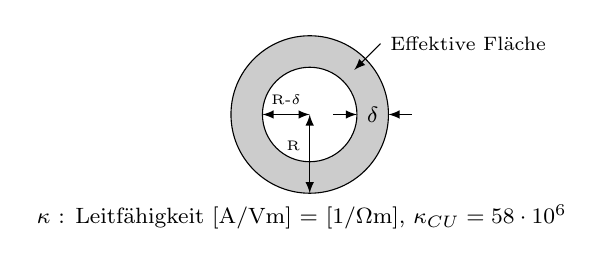
\begin{tikzpicture}
        %Kreise
        \draw[-,fill=black!20] (0,0) circle (1);              %äußerer Kreis
        \draw[-,fill=white] (0,0) circle (0.6);               %innerer Kreis

        %Pfeile
        \draw[latex-latex] (-0.6,0) -- (0,0) node[midway, above]{\tiny{R-$\delta$}};
        \draw[latex-latex] (0,-1) -- (0,0) node at (0,-0.4) [left]{\tiny R};

        \node at (0.8,0)[]{\footnotesize$\delta$};
        \draw[-latex] (0.3,0) -- (0.6,0);
        \draw[latex-] (1,0) -- (1.3,0);

        \draw[latex-] (0.566,0.566) -- (.9,.9) node[above, right]{\scriptsize{Effektive Fläche}};

        %Legende
        \node at (-0.1,-1.3)[]{\footnotesize{$\kappa$ : Leitfähigkeit [A/Vm] = [1/$\Omega$m], $\kappa_{CU} = 58 \cdot 10^6$}};
    \end{tikzpicture}
\end{center}


\begin{description}
    \item Äquivalente Leiterschichtdicke (Amp: $A \cdot \frac{1}{e}$):
          \[
              \delta = \frac{1}{\sqrt{\pi\mu\kappa f}} = \sqrt{\frac{2}{\omega\mu\kappa}} \qquad \left[ m \right] \\
          \]

    \item Widerstand/Oberflächenwiderstand:
        \begin{flalign*}
            R_{AC} & = \frac{l}{\kappa \cdot A_{\texttt{eff}}} \\
            R_{DC} & =\dfrac{l}{\kappa \pi R^{2}}  = \frac{l}{\kappa A}          \\
            R_{OF} & = \dfrac{1}{\kappa \delta}
        \end{flalign*}

    \item \textbf{Feldstärke} verglichen mit der Oberfläche:
    \item analog für $E$-Feld
        \[
            H\left( x,t\right) = H_{0}\cdot e^{^{-x}/_\delta}\cdot \cos \left( \omega t-\dfrac{x}{\delta}\right)\\
        \]  
    \item
        \[
            \hat{H} = \sqrt{\frac{\kappa}{\omega \mu}} \cdot \hat{E}
        \]

    \item \textbf{Leistung} verglichen mit der Oberfläche:
        \[
            P\left( x,t\right) = \dfrac{1}{2} \cdot E_{0}\cdot e^{^{-x}/_\delta}\cdot H_{0}\cdot e^{^{-x}/_\delta}
        \]

    \item Amplitude und Phase bezogen auf $\delta$:
    \item mit $F =$ Dämpfungsfaktor
        \begin{align*}
            \text{Amplitude: } x   & = \ln(F) \qquad \left[\delta\right] \\
            \text{Phase: } \varphi & = -\frac{x}{\delta} \frac{180^{\circ}}{\pi} \qquad \left[^{\circ}\right]
        \end{align*}

    \item Effektive Fläche:
        \begin{align*}
            A_{\texttt{eff}} & = A_{\texttt{ges}} - A_{\kappa} = R^2\pi-(R-\delta)^2\pi \\
                            & = 2\cdot \pi \delta \left( R-\dfrac{\delta }{2}\right)
        \end{align*}
\end{description}

Wenn die Länge nicht gegeben ist oder nach Wieviel \% nimmt der Widerstand bei
einer bestimmten Frequenz, kann dies mit der folgenden Formel berechnet werden:

\begin{description}
    \item Bessel-Funktion:
        \begin{align*}
            \frac{R_{AC}}{R_{DC}} & =
            \begin{dcases}
                1 + \frac{1}{3}x^4              & \text{für} \qquad x < 1 \\
                x + \frac{1}{4} + \frac{3}{64x} & \text{für} \qquad x > 1 \\
            \end{dcases} \\
            \frac{X_{AC}}{R_{DC}} & =
            \begin{dcases}
                x^2\left( 1-\frac{x^4}{6} \right)   & \text{für} \qquad x < 1 \\
                x- \frac{3}{64x} + \frac{3}{128x^2} & \text{für} \qquad x > 1 \\
            \end{dcases}
        \end{align*}
        \[
            \boxed{x=\frac{r_0}{2\delta}} \qquad r_0 \hat{=} \textnormal{Außenradius}
        \]
\end{description}
    \section{Wellen}
$\underline{\gamma}=\alpha+j\beta$\\\\
$\underline{\gamma}$ : Fortpflanzungskonst.\\
$\alpha$ : Dämpfungskonst. [Np/m]\\
$\beta$ : Phasenkonst. [rad/m]\\\\
$v$ : Phasengeschw. [m/s]

\subsection{Ausbreitung}
\subsubsection{Allgemein}
\begin{align*}
     & \alpha = \omega \cdot \sqrt{\dfrac{\mu \varepsilon}{2}\cdot \left(\sqrt{1+\dfrac{\sigma^2}{\omega^2\cdot\varepsilon^2}}-1\right)} \\
     & \beta  = \omega \cdot \sqrt{\dfrac{\mu \varepsilon}{2}\cdot \left(\sqrt{1+\dfrac{\sigma^2}{\omega^2\cdot\varepsilon^2}}+1\right)} \\
     & \underline{Z}_F = \sqrt{\dfrac{j\omega\mu}{\sigma+j\omega\varepsilon}}                                                            \\
     & E_2 = E_1 \cdot e^{-\alpha z}                                                                                                     \\
     & H = \dfrac{E}{Z_F}
\end{align*}

\subsubsection{Im leeren Raum(Vakuum)}
\begin{align*}
     & \alpha = 0                                                                         \\
     & \beta = \dfrac{\omega}{c_0}                                                        \\
     & \underline{Z}_{F0} = \sqrt{\dfrac{\mu_0}{\varepsilon_0}}\text{ }=\text{ }377\Omega \\
     & \lambda = \dfrac{c_0}{f}                                                           \\
     & v = c_0
\end{align*}

\subsubsection{Im Dielektrika mit geringem Verlust}
verlustlos: $\sigma =0$
\begin{align*}
     & \alpha = 0                                                                                                       \\
     & \beta = \dfrac{\omega}{c_0}\cdot\sqrt{\mu_r\varepsilon_r}=\omega\cdot\sqrt{\mu\varepsilon}=\dfrac{2\pi}{\lambda} \\
     & \underline{Z}_F = \sqrt{\dfrac{\mu}{\varepsilon}}                                                                \\
     & \lambda = \dfrac{c_0}{f}\cdot\dfrac{1}{\sqrt{\mu_r\varepsilon_r}}=\dfrac{2\pi}{\beta}                            \\
     & v = \dfrac{c_0}{\sqrt{\mu_r\varepsilon_r}}
\end{align*}

\subsubsection{Im Dielektrika mit geringem Verlust}
geringer Verlust: $0 < \sigma <<\omega\varepsilon$
\begin{align*}
     & \alpha = \dfrac{1}{2}\cdot\sigma\cdot\sqrt{\dfrac{\mu}{\varepsilon}}                                                      \\
     & \beta = \omega\cdot\sqrt{\mu\varepsilon}\cdot\left(1+\dfrac{1}{8}\cdot\dfrac{\sigma^2}{\omega^2\cdot\varepsilon^2}\right) \\
     & \underline{Z}_F = \sqrt{\dfrac{\mu}{\varepsilon}}                                                                         \\
     & \lambda = \dfrac{c_0}{f}\cdot\dfrac{1}{\sqrt{\mu_r\varepsilon_r}}=\dfrac{2\pi}{\beta}                                     \\
     & v = \dfrac{c_0}{\sqrt{\mu_r\varepsilon_r}}
\end{align*}

\subsubsection{Im guten Leiter}
geringer Verlust: $\sigma >>\omega\varepsilon$
\begin{align*}
     & \alpha = \dfrac{1}{\delta}= \beta                                                                                                           \\
    %&\beta = \dfrac{1}{\delta}= \alpha\\
     & \underline{Z}_F = \sqrt{\dfrac{j\omega\mu}{\sigma}} = \sqrt{\dfrac{\omega\mu}{2\sigma}}\cdot\left(1+j\right)=\dfrac{1+j}{\sigma\cdot\delta} \\
     & \lambda = \dfrac{2\pi}{\beta} = 2\pi \sqrt{\dfrac{2}{\omega\mu\sigma}}=2\pi\delta                                                           \\
\end{align*}

\subsection{Übergang}
\subsubsection{Zwischen Dielektrika mit geringem Verlust}
%bitte ergänzen

\subsection{dÀlembertsche Gleichung (allg.)}

\begin{align*}
    \Delta \vec{E}-\kappa \mu \frac{\partial \vec{E}}{\partial t}-\varepsilon \mu \frac{\partial^{2} \vec{E}}{\partial t^{2}} & = \operatorname{grad} \frac{\rho}{\varepsilon} \\
    \Delta \vec{H}-\kappa \mu \frac{\partial \vec{H}}{\partial t}-\varepsilon \mu \frac{\partial^{2} \vec{H}}{\partial t^{2}} & = 0
\end{align*}

Isolator, ideales Dielektrikum, Nichtleiter $\kappa = 0$
\begin{align*}
    \Delta \vec{E} & =\varepsilon \mu \frac{\partial^{2} \vec{E}}{\partial t^{2}}+\operatorname{grad} \frac{\rho}{\varepsilon} \\
    \Delta \vec{H} & =\varepsilon \mu \frac{\partial^{2} \vec{H}}{\partial t^{2}}
\end{align*}

sehr gute Leiter
\begin{align*}
    \Delta \vec{E} & =\kappa \mu \frac{\partial \vec{E}}{\partial t}+\operatorname{grad} \frac{\rho}{\varepsilon} \\
    \Delta \vec{H} & =\kappa \mu \frac{\partial \vec{H}}{\partial t}
\end{align*}

\subsection{Helmholtz-Gleichungen (Frequenzbereich)}
\begin{align*}
    \Delta \underline{\vec{E}}-\left(\kappa \mu \cdot \mathrm{j} \omega-\varepsilon \mu \cdot \omega^{2}\right) \cdot \underline{\vec{E}} & = \operatorname{grad} \frac{\rho}{\varepsilon} \\
    \Delta \underline{\vec{H}}-\left(\kappa \mu \cdot \mathrm{j} \omega-\varepsilon \mu \cdot \omega^{2}\right) \cdot \underline{\vec{H}} & = 0
\end{align*}

\subsubsection{Zeitbereich}
\begin{align*}
    \Delta \vec{E}-\varepsilon \mu \frac{\partial^{2} \vec{E}}{\partial t^{2}} & =0 \\
    \Delta \vec{H}-\varepsilon \mu \frac{\partial^{2} \vec{H}}{\partial t^{2}} & =0
\end{align*}

\subsubsection{Frequenzbereich (harmonisch)}
\begin{align*}
    \Delta \underline{\vec{E}}+\varepsilon \mu \omega^{2} \cdot \underline{\vec{E}} & =0 \\
    \Delta \underline{\vec{H}}+\varepsilon \mu \omega^{2} \cdot \underline{\vec{H}} & =0
\end{align*}

%%%%%%%%%%%%%%%%%

\subsection{Wellenzahl}
Im Vakuum: $k_{0}=\frac{\omega}{c_{0}}$
\begin{align*}
    k & = \frac{\omega}{v_{p h}} = \frac{2 \pi f}{v_{p h}} = |\vec{k}|                                                              \\
      & = \frac{\omega \cdot n}{c_{0}} = n \cdot k_{0}=\frac{1}{\sqrt{\mu_{r} \cdot \varepsilon_{r}}} \cdot k_{0}=k_{r} \cdot k_{0}
\end{align*}

\subsection{Wellenlänge}
\begin{align*}
    \lambda & = \dfrac{2 \pi}{k} = \dfrac{v_{ph}}{f} = [m]                                                                      \\
            & = \lambda_0 \cdot \dfrac{1}{\sqrt{\mu_r \cdot \varepsilon_r}} = \dfrac{\lambda_0}{n} = \dfrac{2 \pi}{n \cdot k_0} \\
            & \lambda_0 = \dfrac{c_0}{f} = \dfrac{2\pi}{k_0}
\end{align*}

\subsection{Phasengeschwindigkeit}
\[
    \dfrac{d z}{d t} = \upsilon_{ph} = \dfrac{\omega}{k} = \frac{1}{\sqrt{ \mu_r \mu_0 \varepsilon_r \varepsilon_0}} \qquad \upsilon_{ph,\textnormal{Medium} \leq c_0}
\]
%\subsection{Ausbreitung im leeren Raum(Vakuum)}
%\[
%    \text{penis}
%\]

\subsubsection{Gruppengeschwindigkeit}
\[
    \upsilon_{g} = \dfrac{d \omega}{d k} = \dfrac{\textnormal{Wegstück der Wellengruppe}}{\textnormal{Laufzeit der Wellengruppe}}
\]

% \subsection{Feldwellenwiderstand}
% allgemein, idealen Dielektrikum\\
% freier Raum
% \begin{align*}
%     \underline{Z}_F    & = \dfrac{\underline{E}_{\textnormal{transversal}}}{\underline{H}_{\textnormal{transversal}}} = \sqrt{\dfrac{\mu}{\varepsilon}} \\
%     \underline{Z}_{F0} & = \sqrt{\dfrac{\mu_0}{\varepsilon_0}} \approx 120\pi \Omega \approx 377 \Omega
% \end{align*}

\subsection{Polarisation}
\begin{tabularx}{0.45\textwidth}{>{\hsize=.3\hsize}X|>{\hsize=.7\hsize}X}
    Lineare     & wenn der Endpunkt des E–Vektors eine Linie     \\
    \hline
    Elliptische & Endpunkt des E-Vektors eine Ellipse beschreibt
\end{tabularx}

    \section{Leitungen}
\subsection{Allgemeine Lösung Leitungsgleichung}
\begin{align*}
    \underline{U}(\ell)  & = U_h e^{\underline{\gamma} \ell} + U_r e^{-\underline{\gamma} \ell} \\
    \underline{I}(\ell)  & = I_h e^{\underline{\gamma} \ell} + I_r e^{-\underline{\gamma} \ell} \\
    \underline{Z}_L     & = \frac{U_h}{I_h} = \sqrt{ \frac{R + j \omega L}{G + j \omega C}}                                                                                   \\
    \underline{\gamma}  & = \alpha + j\beta = \sqrt{(R+j\omega L)\cdot(G+j\omega C)}                                                                                                            \\
    \lambda             & = \frac{2 \pi}{\beta} \qquad v_p = \frac{\omega}{\beta} \\
    l_\texttt{elek.}    & = \beta \cdot l                                                                                                                                     \\
    \alpha              & = \frac{C R+L G}{2 \sqrt{L C}}=\frac{R}{2 Z_L}+\frac{Z_L G}{2}=\alpha_L+\alpha_D \\
    \beta               & = (j) \omega \sqrt{L C}
\end{align*}
\subsubsection{Reflexionsfaktor}
\begin{align*}
    \underline{r}(\ell)     & = \frac{\underline{U}_r(\ell)}{\underline{U}_h(\ell)} = -\frac{\underline{I}_r(\ell)}{\underline{I}_h(\ell)} = \frac{\underline{U}_r(\ell=0) \cdot \mathrm{e}^{-\mathrm{j} \beta \ell}}{\underline{U}_h(\ell=0) \cdot \mathrm{e}^{+\mathrm{j} \beta \ell}} \\
                            & = \underline{r}(\ell=0) \cdot \mathrm{e}^{-2 \underline{\gamma} \ell}=\underline{r}(\ell=0) \cdot \mathrm{e}^{-2 \alpha \ell} \cdot \mathrm{e}^{-\mathrm{j} 2 \beta \ell}\\
                            & = \frac{\frac{Z_L}{\underline{Z}(\ell)}-1}{\frac{Z_L}{\underline{Z}(\ell)}+1} \\
    \underline{r}           & = \frac{\underline{z}_n-1}{\underline{z}_n+1} \qquad \underline{z}_n=\frac{\underline{Z}}{Z_L}\\
    \underline{r}(\ell = 0) & = \frac{\underline{U}_A-\underline{I}_A Z_L}{\underline{U}_A + \underline{I}_A Z_L}=\frac{\underline{Z}_A-Z_L}{\underline{Z}_A+Z_L}=\frac{\frac{\underline{Z}_A}{Z_L}-1}{\frac{\underline{Z}_A}{Z_L}+1}\\
                    \alpha  & = -\frac{\ln(r_A)}{2l} [\si{Np/m}]  \qquad  \beta = \dfrac{\phi_2 -\phi_1}{2l} [\si{rad/m}]
\end{align*}

\subsubsection{Verlustlose Übertragungsleitung }
\begin{align*}
    \beta              & = \omega\sqrt{LC} = \frac{2 \pi}{\lambda} = \frac{\omega}{v_p}\qquad \alpha = 0 \\
    Z_L                & =\frac{U_h}{U_r}       = \sqrt{\frac{L}{C}}                                                                          \\
    v_p                & = \frac{\omega}{\beta} = \frac{1}{\sqrt{LC}}= \frac{1}{\sqrt{\mu\varepsilon}}= \frac{c_0}{\sqrt{\mu_r\varepsilon_r}} \\
    \lambda            & = \frac{2\pi}{\beta}=\frac{1}{f\sqrt{LC}}= \frac{v_p}{f}= \frac{c_0}{f\sqrt{\mu_r\varepsilon_r}}
\end{align*}


\subsection{Übertragungsleitung mit Last}
\begin{center}
\resizebox{\columnwidth}{!}{
        \begin{circuitikz}%[american voltages]
            %Schaltbild
            \draw(0,0)
            to[V,v=$u_G(t)$](0,2)                               %Spannungsquelle
            to[R=$Z_g$](3,2)                                    %Quelleninnenwiderstand
            to[short,o-o](7,2)                                  %Leitung mit Knoten
            to[short](8 ,2)
            to[R=$Z_A$](8,0)                                    %Lastwiderstand
            to[short](7,0)                                      
            to[short,o-o](3,0)                                  %Leitung mit Knoten
            to[short](0,0);   

            %Knoten + Leitung Beschreibung
            \draw(3,2) node[above] {Eingang/Anfang};
            \draw(7,2) node[above] {Ausgang/Ende};
            \draw[decoration={brace},decorate]
                 (3,2.6) -- node[above=6pt] {$\underline{Z}_L$} (7,2.6);
            
            %linke gestrichelte linie
            \draw[dotted](3,0)--(3,-0.5) node[left]{$l=-d$};
            \draw[dotted](3,-0.5)--(3,-1) node[left]{$z=d$};
            \draw[dotted](3,-1)--(3,-1.5);

            %Pfeil in richtung l
            \draw[-latex](3,-0.5) -- (7,-0.5);
            \node at (4,-0.5)[above]{positiv $l$};
            
            %rechte gestrichelte Linue
            \draw[dotted](7,0)--(7,-0.5) node[right]{$l=0$};          
            \draw[dotted](7,-0.5)--(7,-1) node[right]{$z=0$};
            \draw[dotted](7,-1)--(7,-1.5);

            %pfeil in richtung z
            \draw[latex-](3,-1) -- (7,-1);
            \node at (6,-1)[above]{positiv $z$};

            %Pfeil in hinlaufende richtung
            \draw[-latex](3,1.25) -- (6.5,1.25);
            \node at (4.5,1.25)[above]{hinlaufende Welle};

            %Pfeil in rücklaufende richtung
            \draw[latex-](3.5,0.5) -- (7,0.5);
            \node at (5.5,0.5)[above]{rücklaufende Welle};

            %Pfeil Eingangs Widerstand
            \draw[-latex](1,0.5) -- (2.8,0.5);
            \node at (2,0.5)[above]{$\underline{Z}_E$};
        \end{circuitikz}
}
\end{center}



% \subsubsection{Vorgehen Eingangswiderstand}
% Wenn mit Smithdiagramm gearbeitet wird liefert dieses Schritte \ref{Ref L_anfang} und \ref{Bestimmen Z_E}
% \begin{enumerate}
%     \item Lastimpedanz
%           \[ \underline{Z}_A = \dfrac{1}{\frac{1}{R_A} + j \omega C_A} \]
%     \item Reflexion am Leitungsende
%           \[ \underline{r}(z=0) = \dfrac{Z_A - \underline{Z}_L}{Z_A + \underline{Z}_L} \]
%     \item Reflexion am Leitungsanfang \label{Ref L_anfang}
%           \[ \underline{r}(\ell = -d) =  \underline{r}_A \cdot e^{-j 2 \beta d}\]
%     \item Bestimmung der Impedanz \label{Bestimmen Z_E}
%           \[ \underline{Z}_E = \underline{Z}_L \cdot \dfrac{1 + \underline{r}_E}{1 - \underline{r}_E}\]
%     \item Eingangswiderstand
%           \[ \underline{Z}_E = \dfrac{1}{\frac{1}{\underline{Z}_E} + j \omega C_E}\]
% \end{enumerate}

\subsubsection{Fall: Angepasste Leitung}
\begin{align*}
    Z_A          & = Z_L = Z(\ell)                              \\
    r_A          & = 0\qquad\rightarrow\text{reflexionsfrei} \\
    \mathrm{SWR} & = 1                                       \\
    U(\ell)         & = U_h\cdot e ^{j\beta \ell}                  \\
    I(\ell)         & = I_h \cdot e^{j\beta \ell}                  \\
                 & = \frac{U_h}{Z_L}\cdot e^{j\beta \ell}
\end{align*}

\subsubsection{Fall: Kurzgeschlossene Leitung}
\begin{align*}
    Z_A          & = 0                                                                                         \\
    Z(\ell)         & = j Z_L\cdot\tan(\beta \ell)        \qquad\rightarrow\text{rein imaginär}                      \\
    r_A          & = -1                                                                                        \\
    \mathrm{SWR} & = \infty                                                                                    \\
    U(\ell)         & = U_h\cdot 2j\sin(\beta \ell)    \qquad\rightarrow U(\ell=0)=0                                    \\
    \hat{U}_E    & = \hat{U}_{G}\cdot\frac{\underline{Z}_E}{\underline{Z}_{G}+\underline{Z}_E} \\
    I(\ell)         & = U_h\cdot 2\cos(\beta \ell)    \qquad\rightarrow I(\ell=0)=I_A=\frac{2U_h}{Z_L}
\end{align*}

\subsubsection{Fall: Leerlaufende Leitung}
\begin{align*}
    Z_A          & = \infty                                                                         \\
    Z(\ell)         & = -jZ_L\cdot \cot(\beta \ell) \qquad\rightarrow\text{rein imaginär}                 \\
    r_A          & = 1                                                                              \\
    \mathrm{SWR} & = \infty                                                                         \\
    U(\ell)         & = U_h\cdot 2\cos(\beta \ell) \qquad\rightarrow U(\ell=0)=0                             \\
    I(\ell)         & = U_h\cdot 2j\sin(\beta \ell) \qquad\rightarrow I(\ell=0)=I_A = \frac{2\cdot U_h}{Z_L}
\end{align*}

\subsubsection{Fall: Beliebiger Abschluss}
\begin{align*}
    \underline{U}(\ell) &= \underline{U}_A\left[\cos (\beta \ell)+\mathrm{j} \frac{\underline{Z}_L}{\underline{Z}_A} \sin (\beta \ell)\right] \\
    \underline{I}(\ell) &= \underline{I}_A\left[\cos (\beta \ell)+\mathrm{j} \frac{\underline{Z}_A}{\underline{Z}_L} \sin (\beta \ell)\right] \\
    \underline{Z}_E     &= \frac{U(-\ell)}{\underline{I}(-\ell)}= \underline{Z}_A \cdot \frac{1+j \frac{Z_W}{\underline{Z}_A} \tan \beta \ell}{1+j \frac{\underline{Z}_A}{Z_W} \tan \beta \ell} 
\end{align*}
Besonderheit bei $L=\frac{\lambda}{4}$ :
$ \underline{Z}_E=\frac{Z_{W}^2}{\underline{Z}_A}$

\subsubsection{Fall: Ohm'sch abgeschlossene Leitung}
\begin{align*}
                          & r_A = \texttt{reell} \\
    \underline{R_A > Z_L} & \rightarrow\theta_r = 0 \rightarrow r_A \texttt{ ist negativ} \\
                          & \rightarrow \ell_\texttt{max}=\frac{\lambda}{2}\cdot n \\
    \underline{R_A < Z_L} & \rightarrow\theta_r = \pi                           \\
                          & \rightarrow \ell_\texttt{min}=\frac{\lambda}{2}\cdot n
\end{align*}

\subsubsection{Stehwellenverhältnis/ Anpassungsfaktor}
siehe auch Kap. \ref{sec:Smith_All}
\begin{align*}
    \mathrm{SWR}      & = \frac{U_\text{max}}{U_\text{min}} = \frac{I_\text{max}}{I_\text{min}} = \frac{1+|r(\ell)|}{1-|r(\ell)|} = \frac{|U_h|+|U_r|}{|U_h|-|U_r|} \\
    m                 & = \frac{1}{\mathrm{SWR}} = \frac{1 - |r(\ell)|}{1 + |r(\ell)|}
\end{align*}


\subsubsection{vernachlässigbarer Widerstandsbelag}
\includegraphics[width=\columnwidth]{Figures/vernachlaessigbarerWiderstandsbelag.png}

\subsubsection{vernachlässigbarer Leitwertbelag}
\includegraphics[width=\columnwidth]{Figures/vernachlaessigbarerLeiterwertbelag.png}


\subsubsection{Leistung}
\begin{align*}
    P_{A}            & = P_{H}-P_{R}                                                                                                 \\
                     & = \frac{1}{2} \cdot \frac{\hat{U}_{h}^{2}}{Re\{Z_{L}\}}-\frac{1}{2} \cdot \frac{\hat{U}_{r}^{2}}{Re\{Z_{L}\}} \\
                     & =\frac{1}{2} \cdot \frac{\hat{U}_{h}^{2}}{Re\{Z_{L}\}} \cdot\left(1-r^{2}\right)                              \\
                     & = P_{\max} \cdot\left(1-r^{2}\right)                                                                          \\
                     & = \underline{U}_A\cdot\underline{I}_A^*                                                                       \\
    P_V              & = P_q -P_A                                                                                                    \\
    \underline{I}(\ell) & = \hat{I}\cdot e^{-\alpha \ell}\angle \beta \ell
\end{align*}
\subsubsection{Gleichspannungswert (=Endwert)}
\begin{align*}
    U_A & = U_q\cdot\frac{R_A}{R_i+R_A}
\end{align*}

\subsubsection{Position von Extrema}
\begin{align*}
    \lambda_\texttt{min/max}    & = \frac{c_0}{f_\texttt{min/max}\sqrt{\mu_{r1}\varepsilon_{r1}}}\\
    z_\texttt{min}              & =\frac{-n\cdot\lambda_\texttt{min}}{2}                                        \qquad\rightarrow n = -\frac{2z}{\lambda_\texttt{min}}                            \\
    z_\texttt{max}              & =\frac{-(2n+1)\lambda_\texttt{max}}{4}                                        \qquad\rightarrow n = -\frac{4z+\lambda_\texttt{max}}{2\cdot\lambda_\texttt{max}} \\
    z                           & = \frac{\lambda_\texttt{min}\cdot\lambda_\texttt{max}}{4(\lambda_\texttt{min}-\lambda_\texttt{max})}
\end{align*}

\subsection{Mehrfachreflexionen bei fehlender Anpassung}
\begin{center}
    \resizebox{\columnwidth}{!}{
    \begin{tikzpicture}
        %Linien
        \draw[-Latex] (1,1) -- (1,0) node [below] {$t$};
        \draw[-,line width=1pt] (1,1) -- (1,6);
        \draw[-,line width=1pt] (5,0) -- (5,6);

        %Pfeile mit Bezeichnungen
        \draw[-Latex] (3.5,6.5) -- (5,6.5)node[right]{$z$};

        \draw[-Latex] (1,6) -- (5,5) node[right]{$t_d$} node[midway, above]{$u_{1h}$};
        %\draw[-] (1,6) -- (3,5.5) node[above]{$U_{1h}$};

        \draw[-Latex] (5,5) -- (1,4)node[left]{$2\cdot t_d$} node[midway, above]{$u_{1r}$};
        %\draw[-] (5,5) -- (3,4.5) node[above]{$U_{1r}$};

        \draw[-Latex] (1,4) -- (5,3)node[right]{$3\cdot t_d$} node[midway, above]{$u_{2h}$};
        %\draw[-] (1,4) -- (3,3.5) node[above]{$U_{2h}$};

        \draw[-Latex] (5,3) -- (1,2)node[left]{$4\cdot t_d$} node[midway, above]{$u_{2r}$};
        %\draw[-] (5,3) -- (3,2.5) node[above]{$U_{2r}$};

        \draw[-Latex] (1,2) -- (5,1)node[right]{$5\cdot t_d$} node[midway, above]{$u_{3h}$};
        %\draw[-] (1,2) -- (3,1.5) node[above]{$U_{3h}$};


        \draw[dotted ] (5,1) -- (3,0.5);

        %Klammern mit Bezeichnungen
        \draw [black,
            decorate,
            decoration = {brace,
                    raise=5pt,
                    amplitude=5pt}] (5,5.8) --  (5,5.2);
        \node at (5.5,5.5)[right]{$u_A = 0$};

        \draw [black,
            decorate,
            decoration = {brace,
                    raise=5pt,
                    amplitude=5pt}] (1,4.2) --  (1,5.8);
        \node at(0.5,5)[left]{$u_E = u_{1h}$};

        \draw [black,
            decorate,
            decoration = {brace,
                    raise=5pt,
                    amplitude=5pt}] (5,4.8) --  (5,3.2);
        \node at (5.5,4)[right]{$u_A = u_{1h}(1+\underline{r}_A)$};

        \draw [black,
            decorate,
            decoration = {brace,
                    raise=5pt,
                    amplitude=5pt}] (1,2.2) --  (1,3.8);
        \node at (0.5,3)[left]{$u_E = u_{1h}$};
        \node at (0.5,2.5)[left]{$+(1+\underline{r}_I)u_{1r}$};

        \draw [black,
            decorate,
            decoration = {brace,
                    raise=5pt,
                    amplitude=5pt}] (5,2.8) --  (5,1.2);
        \node at (5.5,2)[right]{$u_A = u_{1h}(1+\underline{r}_A)$};
        \node at (5.5,1.5)[right]{$+u_{2h}(1+\underline{r}_A)$};


        \draw [black,
            decorate,
            decoration = {brace,
                    raise=5pt,
                    amplitude=5pt}] (1,0.2) --  (1,1.8);
        \node at (0.5,1.5)[left]{$u_E = u_{1h}$};
        \node at (0.5,1)[left]{$+(1+\underline{r}_I)u_{1r}$};
        \node at (0.5,0.5)[left]{$+(1+\underline{r}_I)u_{2r}$};
    \end{tikzpicture}
    }
\end{center}

\begin{align*}
    %u_{1h} & = u_G\cdot\frac{ Z_L}{R_I + Z_L}            \\
    u_{1r} & = r_A\cdot u_{1h}                                \\
    u_{2h} & = r_I\cdot u_{1r} = r_I\cdot r_A\cdot u_{1h}     \\
    u_{2r} & = r_A\cdot u_{2h} = r_I\cdot r_A^2\cdot u_{1h}   \\
    u_{3h} & = r_I\cdot u_{2r} = r_I^2\cdot r_A^2\cdot u_{1h}
\end{align*}
\input{Figures/Leitungen_Mehrfach_Reflexion_Circuit.tex}
\begin{align*}
     & \text{Reflexionsfaktor Leitungsanfang: } & \underline{r}_I & = \frac{R_I - Z_L}{R_I + Z_L}                 \\
     & \text{Reflexionsfaktor Leitungsende: }   & \underline{r}_A & = \frac{R_A - Z_L}{R_A + Z_L}                 \\
     & \text{Hinlaufende Welle}                 & u_{1h}          & = \hat{u}_G \cdot\frac{Z_L}{Z_L+R_I}          \\
     & \text{Signallaufzeit: }                  & t_d             & = \frac{l}{c_0}\cdot\sqrt{\mu_r\varepsilon_r} \\
     &                                          &                 & = \frac{l}{v_p}
\end{align*}
\subsection{Kettenmatrix einer Leitung}
\[
    A =
    \left[ {\begin{array}{cc}
                    \cosh(\gamma l)               & Z_L \sinh(\gamma l) \\
                    \frac{1}{Z_L} \sinh(\gamma l) & \cosh(\gamma l)     \\
                \end{array} } \right]
\]

\subsection{Leitungsparameter}

{\small\[
        \sigma = \text{Leitwert des Dielektr.} \qquad \sigma_c = \text{Leitwert des Leiters}
    \]}

\subsubsection{Parallele Platten}
{\small\[
        w  = \text{Platten Breite} \qquad d  = \text{Abstand zw. Platten}
    \]}

Für Sinus-Anregung:
\begin{align*}
    I & = \frac{U}{Z_L} = \underbrace{\frac{U_0}{Z_L}}_{I_0}\cdot e^{-j\beta z\cdot e^{j\omega t}}                         \\
    U & = \int \vec{E} d\vec{s} \stackrel{w\gg d}{=} E\cdot d \rightarrow E = \frac{U_0}{d}\cdot^{-j\beta z}\cdot\vec{e}_x \\
    I & = \oint \vec{H} d\vec{s} =  H\cdot w \rightarrow H = \frac{I_0}{w}\cdot^{-j\beta z}\cdot\vec{e}_y                  % \\
    % \vec{E}(r, z) & = \frac{I}{2\pi r}\cdot Z_F\cdot e^{-j\beta z} \cdot\vec{e}_r                                                      \\
    %               & = \frac{\hat{U}}{r \cdot\ln{(^{2b}/_{2a})}}\cdot e^{-j\beta z}\cdot\vec{e}_r
\end{align*}

\input{Figures/Leitungen_Parallele_Platten.tex}
{\renewcommand*{\arraystretch}{0.2}
    \begin{tabularx}{0.5\columnwidth}{|X|}
        \hline
        \[R=\frac{2}{w\delta\sigma}\] \\
        \hline
        \[L=\frac{\mu d}{w}\]         \\
        \hline
        \[G=\frac{\sigma w}{d}\]      \\
        \hline
        \[C=\frac{w\varepsilon}{d}\]  \\
        \hline
    \end{tabularx}
}

\subsubsection{Doppelleitung:}
{\small\[
        a = \text{Leiter Radius} \qquad d = \text{Abstand zw. den Leitern}\\
    \]}
{\small\[
        \text{cosh am TR: MENU $\rightarrow$ 1; OPTN $\rightarrow$ 1 $\rightarrow$ 5}\\
    \]}
\input{Figures/Leitungen_Doppelleitung.tex}
{\renewcommand*{\arraystretch}{0.2}
    \begin{tabularx}{0.5\columnwidth}{|X|}
        \hline
        \[R  = \frac{1}{\pi a\delta\sigma_c}\]              \\
        \hline
        \[L = \frac{\mu}{\pi} \cosh^{-1}\frac{d}{2a}\]      \\
        \hline
        \[G = \frac{\pi\sigma}{\cosh^{-1}(^d/_{2a})}\]      \\
        \hline
        \[C = \frac{\pi\varepsilon}{\cosh^{-1}(^d/_{2a})}\] \\
        \hline
    \end{tabularx}}

\subsubsection{Koaxial Leitung}
{\small\[
        a = \text{innen Radius} \qquad b = \text{außen Radius} \\
    \]}
\begin{align*}
    \vec{H}(r, z)         & = \frac{\hat{I}}{2\pi r}\cdot e^{-j\beta z}\cdot\vec{e}_\varphi                   \\
    \vec{E}(r, z)         & = \frac{\hat{I}}{2\pi r}\cdot Z_{F0}\cdot e^{-j\beta z} \cdot\vec{e}_r
                          & = \frac{\hat{U}}{r \cdot\ln{(^{b}/_{a})}}\cdot e^{-j\beta z}\cdot\vec{e}_r        \\
    \vec{S}_{zeit.Mittel} & = \frac{1}{2}\cdot\left[\frac{\hat{I}}{2\pi r}\right]^2\cdot Z_{F0}\cdot\vec{e}_z
\end{align*}
\input{Figures/Leitungen_Koaxialleitung.tex}
{\renewcommand*{\arraystretch}{0.2}
    \begin{tabularx}{0.5\columnwidth}{|X|}
        \hline
        \[R=\frac{1}{2\pi\delta\sigma_c}\left[\frac{1}{a}+\frac{1}{b}\right]\] \\
        \hline
        \[L=\frac{\mu}{2\pi}\ln\frac{b}{a}\]                                   \\
        \hline
        \[G=\frac{2\pi\sigma}{\ln(^b/_a)}\]                                    \\
        \hline
        \[C=\frac{2\pi\varepsilon}{\ln(^b/_a)}\]                               \\
        \hline
    \end{tabularx}}



\vspace{1ex}
Für beliebige Leitergeometrie gelten folgende Zusammenhänge:
\[
    LC = \mu\varepsilon \quad \text{und} \quad \frac{G}{C} = \frac{\sigma}{\varepsilon}
\]
Innere Induktivität:
\[
    L_i = \frac{R}{w}
\]

\includegraphics[width=1\columnwidth]{Figures/ZahlentabelleLeitungsparameter.png}
    \section{Smith-Diagramm}

\subsection{Allgemein} \label{sec:Smith_All}


$m$             : Anpassungsfaktor

$s$             : inverser Anpassungsfaktor

$\underline{r}$ : Reflexionsfaktor

$1$             : Anpassungspunkt

\begin{center}
    \begin{align*}
        \Aboxed{r(z)  = r_A \cdot e^{-j2\beta z}}                                              \\
        \Aboxed{Z(z)  = Z_L\cdot\frac{Z_A+jZ_L\cdot\tan(\beta z)}{Z_L+jZ_A\cdot\tan(\beta z)}} \\
        \text{mit} \beta = \frac{2\pi}{\lambda}                                                \\
        \text{auch ohne Quelle gültig!}
    \end{align*}
    

\usetikzlibrary{decorations.pathmorphing}
\usetikzlibrary{decorations.text}
\tikzset{
cross/.style={cross out, draw=black, minimum size=2*(#1-\pgflinewidth), inner sep=0pt, outer sep=0pt},
%     %default radius will be 1pt. 
cross/.default={3.5pt}
dot/.style={circle, fill=#1, inner sep=0, minimum size=4pt},
mini dot/.style={circle, inner sep=0pt, minimum size=2pt, pos=1, fill, node contents={}},
}

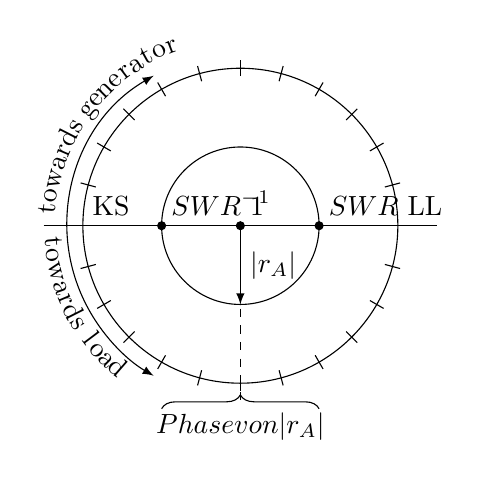
\begin{tikzpicture}
    \draw[-latex](0,0)--(0,-1) node[right, midway]{$|r_A|$};
    \draw[dashed](0,0)--(0,-2.25) node[below]{$\text{Phase von }|r_A|$};
    \draw [black,
        decorate,
        decoration = {brace,
                raise=5pt,
                amplitude=5pt}] (-1,-2.5) --  (1,-2.5);

    \draw[-,fill=black!100] (-1,0) circle (0.05) node[above right]{$\text{\tiny{SWR}}^\text{\tiny{-1}}$};
    \draw[-,fill=black!100] (0,0) circle (0.05);
    \draw[-,fill=black!100] (1,0) circle (0.05) node[above right]{$\text{\tiny{SWR}}$};
    \node at (-2,0)[above right]{KS};
    \node at (0,0)[above right]{1};
    \node at (2,0)[above right]{LL};
    \path (0,0) coordinate (c);
    \draw[-](-2.5,0)--(2.5,0);
    \node[, rotate around={85:(c)}] at (0,2.47){t};
    \node[, rotate around={81:(c)}] at (0,2.44){o};
    \node[, rotate around={76:(c)}] at (0,2.43){w};
    \node[, rotate around={71:(c)}] at (0,2.43){a};
    \node[, rotate around={67:(c)}] at (0,2.43){r};
    \node[, rotate around={63:(c)}] at (0,2.48){d};
    \node[, rotate around={59:(c)}] at (0,2.43){s};

    \node[, rotate around={53:(c)}] at (0,2.39){g};
    \node[, rotate around={49:(c)}] at (0,2.43){e};
    \node[, rotate around={45:(c)}] at (0,2.43){n};
    \node[, rotate around={41:(c)}] at (0,2.43){e};
    \node[, rotate around={37:(c)}] at (0,2.43){r};
    \node[, rotate around={33:(c)}] at (0,2.43){a};
    \node[, rotate around={29:(c)}] at (0,2.47){t};
    \node[, rotate around={25:(c)}] at (0,2.44){o};
    \node[, rotate around={21:(c)}] at (0,2.43){r};

    \node[, rotate around={-85:(c)}] at (0,-2.38){t};
    \node[, rotate around={-81:(c)}] at (0,-2.42){o};
    \node[, rotate around={-76:(c)}] at (0,-2.42){w};
    \node[, rotate around={-71:(c)}] at (0,-2.42){a};
    \node[, rotate around={-67:(c)}] at (0,-2.42){r};
    \node[, rotate around={-63:(c)}] at (0,-2.38){d};
    \node[, rotate around={-59:(c)}] at (0,-2.42){s};

    \node[, rotate around={-53:(c)}] at (0,-2.37){l};
    \node[, rotate around={-49:(c)}] at (0,-2.42){o};
    \node[, rotate around={-45:(c)}] at (0,-2.42){a};
    \node[, rotate around={-41:(c)}] at (0,-2.37){d};

    \draw[-, rotate around={0:(c)}](1.9,0)--(2.1,0);
    \draw[-, rotate around={15:(c)}](1.9,0)--(2.1,0);
    \draw[-, rotate around={30:(c)}](1.9,0)--(2.1,0);
    \draw[-, rotate around={45:(c)}](1.9,0)--(2.1,0);
    \draw[-, rotate around={60:(c)}](1.9,0)--(2.1,0);
    \draw[-, rotate around={75:(c)}](1.9,0)--(2.1,0);
    \draw[-, rotate around={90:(c)}](1.9,0)--(2.1,0);
    \draw[-, rotate around={105:(c)}](1.9,0)--(2.1,0);
    \draw[-, rotate around={120:(c)}](1.9,0)--(2.1,0);
    \draw[-, rotate around={135:(c)}](1.9,0)--(2.1,0);
    \draw[-, rotate around={150:(c)}](1.9,0)--(2.1,0);
    \draw[-, rotate around={165:(c)}](1.9,0)--(2.1,0);
    \draw[-, rotate around={180:(c)}](1.9,0)--(2.1,0);
    \draw[-, rotate around={195:(c)}](1.9,0)--(2.1,0);
    \draw[-, rotate around={210:(c)}](1.9,0)--(2.1,0);
    \draw[-, rotate around={225:(c)}](1.9,0)--(2.1,0);
    \draw[-, rotate around={240:(c)}](1.9,0)--(2.1,0);
    \draw[-, rotate around={255:(c)}](1.9,0)--(2.1,0);
    \draw[-, rotate around={270:(c)}](1.9,0)--(2.1,0);
    \draw[-, rotate around={285:(c)}](1.9,0)--(2.1,0);
    \draw[-, rotate around={300:(c)}](1.9,0)--(2.1,0);
    \draw[-, rotate around={315:(c)}](1.9,0)--(2.1,0);
    \draw[-, rotate around={330:(c)}](1.9,0)--(2.1,0);
    \draw[-, rotate around={345:(c)}](1.9,0)--(2.1,0);
    \draw[-](0,0) circle (1);
    \draw[-](0,0) circle (2);
    \draw[latex-latex](120:2.2) arc (120:240:2.2);

\end{tikzpicture}

\end{center}
\begin{align*}
    \underline{z}_n & = \frac{\underline{Z}_n}{Z_L} = \frac{\underline{r}_n + 1}{\underline{r}_n - 1}                                                                                                                \\
    \underline{r}_n & = \frac{\underline{Z}_n-Z_L}{\underline{Z}_n+Z_L}= \frac{\underline{z}_n-1}{\underline{z}_n+1}    = \frac{1-\underline{y}_n}{1+\underline{y}_n} \\
    m               & = \frac{1-|\underline{r}|}{1+|\underline{r}|}                                                                                                   \\
    s               & = \frac{1}{m}
\end{align*}

\subsection{Impedanz/Admetanz umrechnen}
Im Smithchart spiegeln (Phase $\pm 180^{\circ}$/$\pm \pi$)

\subsection{Maxima/Minima bei stehender Welle}\label{sec:max_min_stehende_welle}
Bei \textbf{verlustloser} Leitung:
\begin{align*}
	 & U_{\texttt{max}} = |U_h| \cdot (1+|r(l)|)                            & U_{\texttt{min}} = |U_h| \cdot (1-|r(l)|)                           & \\
	 & I_{\texttt{max}} = \left | \frac{U_h}{Z_L} \right | \cdot (1+|r(l)|) & I_{\texttt{min}} = \left| \frac{U_h}{Z_L} \right | \cdot (1-|r(l)|) &
\end{align*}

Für \textbf{Spannungen}: Abstand von der Last $ z $: \quad $ n=0,1,2,3... $
\begin{align*}
	                                                                                    & z_{\texttt{min}} = \frac{\lambda}{4\pi}(\theta_{rad}+(2n+1)\pi)                             &
	z_{\texttt{max}} = \frac{\lambda}{4\pi} \cdot (\theta_{rad}+2n\pi)                  &                                                                                               \\
	\Aboxed{                                                                            & \text{\textbf{Minima} alle}\: \frac{\lambda}{2} \rightarrow \frac{l}{\lambda}=0.5} \Aboxed{ &
	\text{\textbf{Maxima} alle}\: \frac{\lambda}{4} \rightarrow \frac{l}{\lambda}=0.25} &
\end{align*}
$ \rightarrow $ Schnittpunkte mit der reellen Achse!\\
Strommaxima sind an Spannungsminima und umgekehrt.

\subsection[Von Last zu Quelle]{Lastseite $\rightarrow$ Quelle}
\begin{enumerate}
    \item $Z_L$ ins Diagramm einzeichen
    \item Lastimpedanz bestimmen,
          wenn zB Parallelschaltung etc
    \item Normieren
          \[\underline{z}_a = \frac{\underline{Z}_A}{Z_L} \]
    \item Ins Chart eintragen
    \item Linie vom Mittelpunkt durch $\underline{z}_a$ nach außen

          Ablesen und Notieren:

          $\rightarrow$Relative Länge $\left[\frac{l}{\lambda}\right]$

          $\rightarrow$Relativer Winkel
    \item Kreis einzeichen

          Ablesen und Notiere:

          $\rightarrow$Maxima: rechter Schnittpunkt mit Re-Achse

          $\rightarrow$Minima: linker  Schnittpunkt mit Re-Achse

          $\rightarrow$Rexlexionsfaktor abmessen und aus Skala oben auslesen
    \item Um Leitungslänge im UZS laufen
          $\rightarrow$ Linie vom Mittelpunkt durch neuen Punkt nach außen

          Ablesen und Notieren:

          $\rightarrow$Relativer Winkel
    \item Wenn $\alpha\neq 0$

          $\rightarrow$ Dämpung ausrechen
          $\rightarrow$ Um Faktor nach innen Spiralieren

    \item Dieser Punkt ist $\underline{z}_e$
    \item Eingangsimpedanz ablesen
          \[\underline{Z}_E = \underline{z}_e \cdot Z_L\]
\end{enumerate}

\subsection{Vorgehen mit geg. Eingangswiderstand}
Wenn mit dem Smith-Diagramm gearbeitet wird, liefert dies die Schritte
\ref{Ref L_anfang} und \ref{Bestimmen Z_E}
\begin{enumerate}
	\item Lastimpedanz
	      \[ \underline{Z}_A = \dfrac{1}{\frac{1}{R_A} + j \omega C_A} \]
	\item Reflexion am Leitungsende
	      \[ \underline{r}_A = \underline{r}(z=0) = \dfrac{Z_A - \underline{Z}_L}{Z_A + \underline{Z}_L} \]
	\item Reflexion am Leitungsanfang \label{Ref L_anfang}
	      \[ \underline{r}_E = \underline{r}(z=d) =  \underline{r}_A \cdot e^{-j 2 \beta d}\]
	\item Bestimmung der Impedanz \label{Bestimmen Z_E}
	      \[ \underline{Z}_E = \underline{Z}_L \cdot \dfrac{1 + \underline{r}_E}{1 - \underline{r}_E}\]
	\item Eingangswiderstand
	      \[ \underline{Z}_E = \dfrac{1}{\frac{1}{\underline{Z}_E} + j \omega C_E}\]
\end{enumerate}


\usetikzlibrary{decorations.pathmorphing}
\usetikzlibrary{decorations.text}
\tikzset{
cross/.style={cross out, draw=black, minimum size=2*(#1-\pgflinewidth), inner sep=0pt, outer sep=0pt},
%     %default radius will be 1pt. 
cross/.default={3.5pt}
dot/.style={circle, fill=#1, inner sep=0, minimum size=4pt},
mini dot/.style={circle, inner sep=0pt, minimum size=2pt, pos=1, fill, node contents={}},
}
\begin{center}
 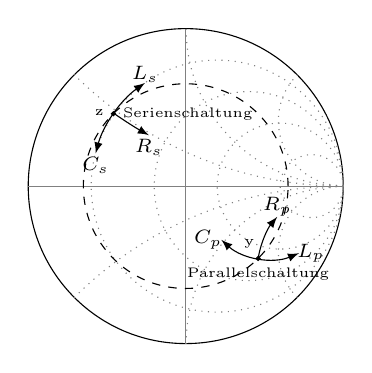
\begin{tikzpicture}    
    
    %Außenkreis
    \draw[-](0,0) circle (2);

    %Realteil Linien
    \draw[-, black!50](-2,0)--(2,0);

    \draw[dotted, black!50](0.4,0) circle (1.6);
    \draw[dotted, black!50](0.8,0) circle (1.2);
    \draw[dotted, black!50](1.2,0) circle (0.8);
    \draw[dotted, black!50](1.6,0) circle (0.4); 

    
    %Imaginärteil Linien
    \draw[-, black!50](0,-2)--(0,2);

    \draw[dotted, black!50, xshift = 13.25ex, yshift = -31.98ex](135:4.84)arc(135:90:4.84);
    \draw[dotted, black!50, xshift = 13.25ex, yshift = -13.25ex](180:2)   arc(180:90:2);
    \draw[dotted, black!50, xshift = 13.25ex, yshift = -5.485ex](225:.828)arc(225:90:.828);

    \draw[dotted, black!50, xshift = 13.25ex, yshift = 31.98ex](270:4.84)arc(270:225:4.84);
    \draw[dotted, black!50, xshift = 13.25ex, yshift = 13.25ex](270:2)   arc(270:180:2);
    \draw[dotted, black!50, xshift = 13.25ex, yshift = 5.485ex](270:.828)arc(270:135:.828);

    %Reflexionsfaktorkreis
    \draw[dashed](0,0) circle (1.3);

    %Serienschaltung
    \draw[-,fill=black!100] (-.919,.919) circle (0.025)node[left, yshift =.5] {\tiny z}node[right]{\tiny Serienschaltung};
    \draw[latex-latex, xshift = 2.65ex](125:1.6)node[above, yshift=-.75ex]{\scriptsize${L_s}$} arc (125:165:1.6)node[below, yshift=.5ex]{\scriptsize$C_s$};
    \draw[latex-, xshift = 13.25ex, yshift = 33.75ex](241:5.1)node[below, yshift=.5ex]{\scriptsize$R_s$}arc(241:235:5.1);

    %Parallelschaltung
    \draw[-,fill=black!100] (.919,-.919) circle (0.025)node[above left, xshift = .5ex]{\tiny y} node[below]{\tiny Parallelschaltung};
    \draw[-latex, xshift = 13.25ex, yshift = -7.25ex](170:1.1)arc(170:140:1.1)node[above, yshift=-.75ex]{\scriptsize$R_p$};

    \draw[latex-latex, xshift = 7.12ex](293:.925)node[right, xshift = -.95ex]{\scriptsize$L_p$}arc(293:227.5:.925)node[left, xshift = .85ex]{\scriptsize$C_p$};

\end{tikzpicture}
\end{center}  
    \include{Wellenleiter}
    \section{Antennen}
\subsection{Herz'scher Dipol}
\boxed{\vec{p} = Q\cdot\vec{d}}
\subsubsection{Allgemein}

{\footnotesize\begin{empheq}[box=\fbox]{align*}
        {\vec{H}} & =-\frac{I_0\Delta l'\beta^2}{4\pi}e^{-j\beta R}\cdot\sin\theta\left(\frac{1}{j\beta R}+\frac{1}{(j\beta R)^2}\right)\vec{e}_\phi                                 \\
        {\vec{E}} & = -\frac{Z_F I_0\Delta l'\beta^2}{2\pi}e^{-j\beta R}\cdot\cos\theta\left(\frac{1}{(j\beta R)^2}+\frac{1}{(j\beta R)^3}\right)\vec{e}_R                           \\
        & = -\frac{Z_F I_0\Delta l'\beta^2}{4\pi}e^{-j\beta R}\cdot\sin\theta\left(\frac{1}{(j\beta R)}+\frac{1}{(j\beta R)^2}+\frac{1}{(j\beta R)^3}\right)\vec{e}_\theta
    \end{empheq}}%

\subsubsection[Nahfeld]{Nahfeld(Fresnel-Zone):\\ $\frac{\lambda}{2\pi R}\gg 1$ oder $\beta R \ll 1$}

Überwiegend \textbf{Blindleistungsfeld}, da $E$ zu $H$ $90^\circ$
phasenverschoben
\begin{empheq}[box=\fbox]{align*}
    \vec{H} & \approx \frac{I_0 \Delta l'}{4\pi R^2}\cdot\sin\theta\cdot\vec{e}_\phi                                            \\
    \vec{E} & \approx \frac{I_0 \Delta l'}{2\pi j \omega\varepsilon R^3}\cos\theta\cdot\vec{e}_R\\
    & +       \frac{I_0 \Delta l'}{4\pi j \omega\varepsilon R^3}\sin\theta\cdot\vec{e}_\theta
\end{empheq}

\subsubsection[Fernfeld]{Fernfeld(Fraunhofer-Zone):\\ $\frac{\lambda}{2\pi R}\ll 1$ oder $\beta R\gg 1$}

Überwiegend \textbf{Wirkleistungsfeld}, $\vec{S}$ nach außen somit Kugelwelle

\vspace{1ex}
mit $\eta = Z_{F0}$

\begin{empheq}[box=\fbox] {align*}
    H & \approx  j\frac{\beta I_0 \Delta l'}{4\pi R}\cdot e^{-j\beta R}\cdot\sin\theta\cdot\vec{e}_\phi                           \\
    E & \approx  j\frac{\beta Z_F I_0 \Delta l'}{4\pi R}\cdot e^{-j\beta R}\cdot\sin\theta\cdot \vec{e}_\theta
\end{empheq}

\subsubsection{Abgestrahlte Leistung im Fernfeld}
\begin{align*}
    P_\texttt{rad} & = \frac{Z_{F0} {I_0}^2 \beta^2 (\Delta l')^2}{12\pi}                             \\
                   & = \frac{I_0^2 Z_F\pi}{3}\cdot \dfrac{\Delta l'^2}{\lambda^2}                     \\
                   & = 40\pi^2\Omega\cdot\left(\frac{I_0\Delta l'}{\lambda}\right)^2                  \\
    S_{av}         & = \frac{Z_FI_0^2\beta^2(\Delta l')^2}{32\pi^2R^2}\cdot\sin^2\theta\cdot\vec{e}_R \\
                   & = \frac{1}{2}\Re\left\{\vec{E}\times\vec{H}^*\right\}
\end{align*}
\subsubsection{Strahlungswiderstand}
\begin{align*}
    R_{S} & = \frac{2}{3}\pi Z_F\left(\frac{\Delta l'}{\lambda}\right)^2
    = 80\pi^2\Omega\left(\frac{\Delta l'}{\lambda}\right)^2
\end{align*}
\subsubsection{Verlustwiderstand}
\begin{align*}
    R_{v} & = \frac{l}{\sigma\cdot A_\delta}
\end{align*}
\subsection{Magnetischer Dipol}
\boxed{\vec{m} = \vec{I}\pi\vec{a}^2\vec{e}_z}
\boxed{m = I\cdot A}
\begin{center}
    \input{Figures/Antennen_Magnetischer_Dipol.tex}
\end{center}

\begin{align*}
    \vec{A}  & = \frac{\mu m}{4\pi R^2}(1+j\beta R) e^{-j\beta R}\sin\theta\cdot\vec{e}_\phi \\
    \Delta l & \rightarrow \beta\pi\ a^2
\end{align*}

{\footnotesize\begin{empheq}[box=\fbox]{align*}
    {\vec{H}}   & = -\frac{j\omega\mu\beta^2m}{2\pi Z_{F0}}e^{-j\beta R}\cdot\cos\theta\left(\frac{1}{(j\beta R)^2}+\frac{1}{(j\beta R)^3}\right)\vec{e}_R                             \\
    & = -\frac{j\omega\mu\beta^2m}{4\pi Z_{F0}}e^{-j\beta R}\cdot\sin\theta\left(\frac{1}{(j\beta R)}+\frac{1}{(j\beta R)^2}+\frac{1}{(j\beta R)^3}\right)\vec{e}_\theta   \\
    {\vec{E}}   & =  \frac{j\omega\mu\beta^2m}{4\pi}e^{-j\beta R}\sin\theta\left(\frac{1}{j\beta R}+\frac{1}{(j\beta R)^2}\right)\vec{e}_\phi
\end{empheq}}%

\subsubsection{Fernfeld}
\begin{empheq}[box=\fbox]{align*}
    E & \approx -\frac{\beta m\omega\mu}{4\pi R}e^{-j\beta R}\sin\theta\cdot\vec{e}_\phi \\
    H & \approx -\frac{\beta m\omega\mu}{4\pi R Z_{F0}}e^{-j\beta R}\sin\theta\cdot\vec{e}_\theta
\end{empheq}
\subsubsection{Abgestrahlte Leistung im Fernfeld}
\begin{align*}
    P_\texttt{rad} & = \frac{Z_F\beta^4m^2}{12\pi}                                     \\
                   & = \frac{m^2\mu\omega^4}{12\pi v_p^3}                              \\
    S_{av}         & = \frac{Z_F\beta^4m^2}{32\pi^2R^2}\cdot\sin^2\theta\cdot\vec{e}_R \\
                   & = \frac{1}{2}\Re\left\{\vec{E}\times\vec{H}^*\right\}
\end{align*}

\subsubsection{Nahfeld}
\begin{empheq}[box=\fbox]{align*}
    E & \approx -\frac{jm\omega\mu}{4\pi R^2}\sin\theta\cdot\vec{e}\phi \\
    H & \approx \frac{m}{4\pi R^3}(2\cos\theta\cdot\vec{e}_R+\sin\theta\cdot\vec{e}_\theta)
\end{empheq}

\subsection{Lineare Antenne}
\begin{align*}
    I(z') & = I_0\cdot\sin\left[\beta\left(\frac{L}{2}-|z'|\right)\right]
\end{align*}

\subsubsection{Dipolantenne}
\begin{align*}
    \vec{H}      & = j\cdot\frac{I_0}{2\pi R}\cdot e^{-j\beta R}\cdot\frac{\cos\left[\left(\frac{\beta L}{2}\right)\cos\theta\right]-\cos\left(\frac{\beta L}{2}\right)}{\sin\theta}\cdot\vec{e}_\phi         \\
    \vec{E}      & = H\cdot Z_F\cdot\vec{e}_\theta                                                                                                                                                            \\
    I_0          & = \sqrt{\frac{2\cdot P_{Send}}{R_S}}                                                                                                                                                       \\
                 & \text{Die mittlere Strahlungsleistungsdichte}                                                                                                                                              \\
    \vec{S}_{av} & = \frac{Z_FI_0^2}{8\pi^2 R^2}\left(\frac{\cos\left(\frac{\beta L}{2}\cos\theta\right)-\cos\left(\frac{\beta L}{2}\right)}{\sin\theta}\right)^2\cdot\vec{e}_R                               \\
                 & \text{Die gesamte Strahlungsleistung}                                                                                                                                                      \\
    P_S          & = \frac{Z_{F0}I_0^2}{4\pi}\int^{\theta=\pi}_{\theta=0}\frac{\left(\cos\left(\frac{\beta L}{2}\cos\theta\right)-\cos\left(\frac{\beta L}{2}\right)\right)^2}{\sin\theta}\cdot\vec{e}_\theta \\
                 & = \int_A S_{AV}\cdot d\vec{a}                                                                                                                                                              \\
                 & = \int^{2\pi}_{\Phi = 0}\int^{\pi}_{\Theta = 0} S_{AV} R^2 \sin\Theta \cdot d\Theta \cdot d\Phi
\end{align*}

\subsection{Antennenkenngrößen}

\input{Figures/Antennen_Antennenkenngroessen_circuit.tex}

\subsubsection{Abgestrahlte Leistung}
\begin{align*}
    P_S & = \frac{1}{2}\cdot I_A^2 \cdot R_S
\end{align*}

\subsubsection{Verlustleistung}
\begin{align*}
    P_V & = \frac{1}{2}\cdot I_A^2\cdot R_V
\end{align*}

\subsubsection{Wirkungsgrad}
\begin{align*}
    \eta & = \frac{P_S}{P_S + P_V} = \frac{R_S}{R_S + R_V}
\end{align*}

\subsubsection{Richtcharakteristik}
$C_{i} \ent$ isotroper Kugelstrahler als Bezugsgröße in Hauptabstrahlrichtung
\begin{align*}
    C(\vartheta, \varphi)     & = \frac{E(\vartheta, \varphi)}{E_{\max}}=\frac{H(\vartheta, \varphi)}{H_{\max}} = \frac{U(\varphi,\vartheta)}{U_{\max}} & 0 \leq C(\vartheta, \varphi) \leq 1 \\
    C_{i}(\vartheta, \varphi) & = \frac{E(\vartheta, \varphi)}{E_{i}}=\frac{H(\vartheta, \varphi)}{H_{i}}                                               & C_{i}>1
\end{align*}

\subsubsection{Richtfunktion/Richtfaktor}
In $[\si{dB}]$ angeben!
\begin{align*}
    D(\vartheta, \varphi) & = \frac{S(\vartheta, \varphi)}{S_{i}}                               \\
    D(\vartheta, \varphi) & = C_{i}^{2}(\vartheta, \varphi) = D \cdot C^{2}(\vartheta, \varphi) \\
    D                     & = \max \{D(\vartheta, \varphi)\} = \frac{S_{\max}}{S_{i}}
\end{align*}

\subsubsection{Gewinn}
\begin{align*}
    G & = \eta \cdot D \qquad [\si{dB}] \\
\end{align*}

\subsubsection{Wirksame Antennenfläche}
\begin{align*}
    A_\texttt{eff} & = \frac{\lambda^2}{4\pi}\cdot G = \dfrac{Z_{F0}}{4 R_S} \cdot l_\texttt{eff}^2
\end{align*}

\subsection{Bezugsantennen}
\[
    \boxed{g = 10 \cdot log(G) \si{dB}}
\]

mit $P_0$ : Eingangsleistung der Antenne

\begin{description}
    \item \textbf{\underline{G$\rightarrow$Bezugsantenne:}}

          Elementardipol  zu Kugelstrahler \[D = 1,50 \rightarrow g = 1,76\si{dBi}\]
          Halbwellendipol zu Kugelstrahler \[D = 1,64 \rightarrow g = 2,15\si{dBi}\]

    \item \textbf{\underline{EIRP}: Eqivalent \underline{Isoropic} Radiated Power}
          \[
              \text{EIRP} = P_0 \cdot G_i [\si{dBi}]
          \]

    \item \textbf{\underline{ERP}: Eqivalent Radiated Power (verlustloser Halbwellendipol)}
          \[
              \text{ERP} = P_0 \cdot G_d [\si{dBd}]
          \]
\end{description}

\subsection{Senden und Empfangen}
\begin{center}
    \resizebox{0.75\columnwidth}{!}{
        \begin{circuitikz}
            %Schaltbild
            \draw(0,0) node[below right]{$U_0=l_{\texttt{eff}}\cdot E$}
            to[V,v=$U_0 $](0,2)                               %Spannungsquelle
            to[R=$R_{S}$](2,2)                                   %Strahlungswiderstand
            to[short](4 ,2)
            to[R= $R_{E}$](4,0)
            to[short](0,0);
            \draw(3,2) node[below]{$l$}
            to[open,o-o](3,0) node[above]{$l'$};

        \end{circuitikz}
    }
\end{center}


\begin{description}
    \item Senden = transmit = TX
    \item Empfangen = receive = RX
\end{description}

\begin{align*}
    \frac{P_{RX}}{P_{TX}}          & = A_{\texttt{eff},RX}\cdot A_{\texttt{eff},TX}\cdot\frac{1}{\lambda^2r^2}                          \\
                                   & = D_{i,RX}\cdot\eta_{RX}\cdot D_{i,TX}\cdot\eta_{TX}\cdot\left(\frac{\lambda}{4\pi r}\right)^2     \\
    \Aboxed{A_\texttt{eff}(\theta) & = G_{RX}\cdot\frac{\lambda^2}{4\pi}\overbrace{\cdot\frac{3}{2}\cdot\sin^2\theta}^{{D_{i,\theta}}}} \\
    P_{RX}                         & = S_{RX}\cdot A_\texttt{eff}                                                                       \\
                                   & = P_{TX}\cdot G_{TX}\cdot G_{RX}\cdot \left(\frac{\lambda}{4\pi r}\right)^2
\end{align*}

\subsubsection{Freiraumdämpfung/Freiraumdämpfungsmaß}
\begin{align*}
    F = \dfrac{P_{TX}}{P_{RX}} \cdot \left(\dfrac{4 \pi d}{\lambda}\right)^2                         & \qquad [1]       \\
    a_{0} = 20 \lg \left(\frac{4 \pi d}{\lambda}\right) =20 \lg \left(\frac{4 \pi d f}{c_{0}}\right) & \qquad [\si{dB}]
\end{align*}

\subsubsection{Leistungspegel/Freiraumpegel}
\begin{align*}
    L      & = 10 \lg \left(\frac{P}{1 \si{mW}}\right) \qquad [\si{dBm}] \\
    L_{RX} & = L_{TX}+g_{TX}+g_{RX}-a_{0} \qquad [\si{dB}]
\end{align*}

\end{multicols*}
\include{Antennentabelle}

%für Leitungsparameter Grafik von Sattler füllt eine Seite
% \section{Leitungen}
\subsection{Allgemeine Lösung Leitungsgleichung}
\begin{align*}
    \underline{U}(\ell)  & = U_h e^{\underline{\gamma} \ell} + U_r e^{-\underline{\gamma} \ell} \\
    \underline{I}(\ell)  & = I_h e^{\underline{\gamma} \ell} + I_r e^{-\underline{\gamma} \ell} \\
    \underline{Z}_L     & = \frac{U_h}{I_h} = \sqrt{ \frac{R + j \omega L}{G + j \omega C}}                                                                                   \\
    \underline{\gamma}  & = \alpha + j\beta = \sqrt{(R+j\omega L)\cdot(G+j\omega C)}                                                                                                            \\
    \lambda             & = \frac{2 \pi}{\beta} \qquad v_p = \frac{\omega}{\beta} \\
    l_\texttt{elek.}    & = \beta \cdot l                                                                                                                                     \\
    \alpha              & = \frac{C R+L G}{2 \sqrt{L C}}=\frac{R}{2 Z_L}+\frac{Z_L G}{2}=\alpha_L+\alpha_D \\
    \beta               & = (j) \omega \sqrt{L C}
\end{align*}
\subsubsection{Reflexionsfaktor}
\begin{align*}
    \underline{r}(\ell)     & = \frac{\underline{U}_r(\ell)}{\underline{U}_h(\ell)} = -\frac{\underline{I}_r(\ell)}{\underline{I}_h(\ell)} = \frac{\underline{U}_r(\ell=0) \cdot \mathrm{e}^{-\mathrm{j} \beta \ell}}{\underline{U}_h(\ell=0) \cdot \mathrm{e}^{+\mathrm{j} \beta \ell}} \\
                            & = \underline{r}(\ell=0) \cdot \mathrm{e}^{-2 \underline{\gamma} \ell}=\underline{r}(\ell=0) \cdot \mathrm{e}^{-2 \alpha \ell} \cdot \mathrm{e}^{-\mathrm{j} 2 \beta \ell}\\
                            & = \frac{\frac{Z_L}{\underline{Z}(\ell)}-1}{\frac{Z_L}{\underline{Z}(\ell)}+1} \\
    \underline{r}           & = \frac{\underline{z}_n-1}{\underline{z}_n+1} \qquad \underline{z}_n=\frac{\underline{Z}}{Z_L}\\
    \underline{r}(\ell = 0) & = \frac{\underline{U}_A-\underline{I}_A Z_L}{\underline{U}_A + \underline{I}_A Z_L}=\frac{\underline{Z}_A-Z_L}{\underline{Z}_A+Z_L}=\frac{\frac{\underline{Z}_A}{Z_L}-1}{\frac{\underline{Z}_A}{Z_L}+1}\\
                    \alpha  & = -\frac{\ln(r_A)}{2l} [\si{Np/m}]  \qquad  \beta = \dfrac{\phi_2 -\phi_1}{2l} [\si{rad/m}]
\end{align*}

\subsubsection{Verlustlose Übertragungsleitung }
\begin{align*}
    \beta              & = \omega\sqrt{LC} = \frac{2 \pi}{\lambda} = \frac{\omega}{v_p}\qquad \alpha = 0 \\
    Z_L                & =\frac{U_h}{U_r}       = \sqrt{\frac{L}{C}}                                                                          \\
    v_p                & = \frac{\omega}{\beta} = \frac{1}{\sqrt{LC}}= \frac{1}{\sqrt{\mu\varepsilon}}= \frac{c_0}{\sqrt{\mu_r\varepsilon_r}} \\
    \lambda            & = \frac{2\pi}{\beta}=\frac{1}{f\sqrt{LC}}= \frac{v_p}{f}= \frac{c_0}{f\sqrt{\mu_r\varepsilon_r}}
\end{align*}


\subsection{Übertragungsleitung mit Last}
\begin{center}
\resizebox{\columnwidth}{!}{
        \begin{circuitikz}%[american voltages]
            %Schaltbild
            \draw(0,0)
            to[V,v=$u_G(t)$](0,2)                               %Spannungsquelle
            to[R=$Z_g$](3,2)                                    %Quelleninnenwiderstand
            to[short,o-o](7,2)                                  %Leitung mit Knoten
            to[short](8 ,2)
            to[R=$Z_A$](8,0)                                    %Lastwiderstand
            to[short](7,0)                                      
            to[short,o-o](3,0)                                  %Leitung mit Knoten
            to[short](0,0);   

            %Knoten + Leitung Beschreibung
            \draw(3,2) node[above] {Eingang/Anfang};
            \draw(7,2) node[above] {Ausgang/Ende};
            \draw[decoration={brace},decorate]
                 (3,2.6) -- node[above=6pt] {$\underline{Z}_L$} (7,2.6);
            
            %linke gestrichelte linie
            \draw[dotted](3,0)--(3,-0.5) node[left]{$l=-d$};
            \draw[dotted](3,-0.5)--(3,-1) node[left]{$z=d$};
            \draw[dotted](3,-1)--(3,-1.5);

            %Pfeil in richtung l
            \draw[-latex](3,-0.5) -- (7,-0.5);
            \node at (4,-0.5)[above]{positiv $l$};
            
            %rechte gestrichelte Linue
            \draw[dotted](7,0)--(7,-0.5) node[right]{$l=0$};          
            \draw[dotted](7,-0.5)--(7,-1) node[right]{$z=0$};
            \draw[dotted](7,-1)--(7,-1.5);

            %pfeil in richtung z
            \draw[latex-](3,-1) -- (7,-1);
            \node at (6,-1)[above]{positiv $z$};

            %Pfeil in hinlaufende richtung
            \draw[-latex](3,1.25) -- (6.5,1.25);
            \node at (4.5,1.25)[above]{hinlaufende Welle};

            %Pfeil in rücklaufende richtung
            \draw[latex-](3.5,0.5) -- (7,0.5);
            \node at (5.5,0.5)[above]{rücklaufende Welle};

            %Pfeil Eingangs Widerstand
            \draw[-latex](1,0.5) -- (2.8,0.5);
            \node at (2,0.5)[above]{$\underline{Z}_E$};
        \end{circuitikz}
}
\end{center}



% \subsubsection{Vorgehen Eingangswiderstand}
% Wenn mit Smithdiagramm gearbeitet wird liefert dieses Schritte \ref{Ref L_anfang} und \ref{Bestimmen Z_E}
% \begin{enumerate}
%     \item Lastimpedanz
%           \[ \underline{Z}_A = \dfrac{1}{\frac{1}{R_A} + j \omega C_A} \]
%     \item Reflexion am Leitungsende
%           \[ \underline{r}(z=0) = \dfrac{Z_A - \underline{Z}_L}{Z_A + \underline{Z}_L} \]
%     \item Reflexion am Leitungsanfang \label{Ref L_anfang}
%           \[ \underline{r}(\ell = -d) =  \underline{r}_A \cdot e^{-j 2 \beta d}\]
%     \item Bestimmung der Impedanz \label{Bestimmen Z_E}
%           \[ \underline{Z}_E = \underline{Z}_L \cdot \dfrac{1 + \underline{r}_E}{1 - \underline{r}_E}\]
%     \item Eingangswiderstand
%           \[ \underline{Z}_E = \dfrac{1}{\frac{1}{\underline{Z}_E} + j \omega C_E}\]
% \end{enumerate}

\subsubsection{Fall: Angepasste Leitung}
\begin{align*}
    Z_A          & = Z_L = Z(\ell)                              \\
    r_A          & = 0\qquad\rightarrow\text{reflexionsfrei} \\
    \mathrm{SWR} & = 1                                       \\
    U(\ell)         & = U_h\cdot e ^{j\beta \ell}                  \\
    I(\ell)         & = I_h \cdot e^{j\beta \ell}                  \\
                 & = \frac{U_h}{Z_L}\cdot e^{j\beta \ell}
\end{align*}

\subsubsection{Fall: Kurzgeschlossene Leitung}
\begin{align*}
    Z_A          & = 0                                                                                         \\
    Z(\ell)         & = j Z_L\cdot\tan(\beta \ell)        \qquad\rightarrow\text{rein imaginär}                      \\
    r_A          & = -1                                                                                        \\
    \mathrm{SWR} & = \infty                                                                                    \\
    U(\ell)         & = U_h\cdot 2j\sin(\beta \ell)    \qquad\rightarrow U(\ell=0)=0                                    \\
    \hat{U}_E    & = \hat{U}_{G}\cdot\frac{\underline{Z}_E}{\underline{Z}_{G}+\underline{Z}_E} \\
    I(\ell)         & = U_h\cdot 2\cos(\beta \ell)    \qquad\rightarrow I(\ell=0)=I_A=\frac{2U_h}{Z_L}
\end{align*}

\subsubsection{Fall: Leerlaufende Leitung}
\begin{align*}
    Z_A          & = \infty                                                                         \\
    Z(\ell)         & = -jZ_L\cdot \cot(\beta \ell) \qquad\rightarrow\text{rein imaginär}                 \\
    r_A          & = 1                                                                              \\
    \mathrm{SWR} & = \infty                                                                         \\
    U(\ell)         & = U_h\cdot 2\cos(\beta \ell) \qquad\rightarrow U(\ell=0)=0                             \\
    I(\ell)         & = U_h\cdot 2j\sin(\beta \ell) \qquad\rightarrow I(\ell=0)=I_A = \frac{2\cdot U_h}{Z_L}
\end{align*}

\subsubsection{Fall: Beliebiger Abschluss}
\begin{align*}
    \underline{U}(\ell) &= \underline{U}_A\left[\cos (\beta \ell)+\mathrm{j} \frac{\underline{Z}_L}{\underline{Z}_A} \sin (\beta \ell)\right] \\
    \underline{I}(\ell) &= \underline{I}_A\left[\cos (\beta \ell)+\mathrm{j} \frac{\underline{Z}_A}{\underline{Z}_L} \sin (\beta \ell)\right] \\
    \underline{Z}_E     &= \frac{U(-\ell)}{\underline{I}(-\ell)}= \underline{Z}_A \cdot \frac{1+j \frac{Z_W}{\underline{Z}_A} \tan \beta \ell}{1+j \frac{\underline{Z}_A}{Z_W} \tan \beta \ell} 
\end{align*}
Besonderheit bei $L=\frac{\lambda}{4}$ :
$ \underline{Z}_E=\frac{Z_{W}^2}{\underline{Z}_A}$

\subsubsection{Fall: Ohm'sch abgeschlossene Leitung}
\begin{align*}
                          & r_A = \texttt{reell} \\
    \underline{R_A > Z_L} & \rightarrow\theta_r = 0 \rightarrow r_A \texttt{ ist negativ} \\
                          & \rightarrow \ell_\texttt{max}=\frac{\lambda}{2}\cdot n \\
    \underline{R_A < Z_L} & \rightarrow\theta_r = \pi                           \\
                          & \rightarrow \ell_\texttt{min}=\frac{\lambda}{2}\cdot n
\end{align*}

\subsubsection{Stehwellenverhältnis/ Anpassungsfaktor}
siehe auch Kap. \ref{sec:Smith_All}
\begin{align*}
    \mathrm{SWR}      & = \frac{U_\text{max}}{U_\text{min}} = \frac{I_\text{max}}{I_\text{min}} = \frac{1+|r(\ell)|}{1-|r(\ell)|} = \frac{|U_h|+|U_r|}{|U_h|-|U_r|} \\
    m                 & = \frac{1}{\mathrm{SWR}} = \frac{1 - |r(\ell)|}{1 + |r(\ell)|}
\end{align*}


\subsubsection{vernachlässigbarer Widerstandsbelag}
\includegraphics[width=\columnwidth]{Figures/vernachlaessigbarerWiderstandsbelag.png}

\subsubsection{vernachlässigbarer Leitwertbelag}
\includegraphics[width=\columnwidth]{Figures/vernachlaessigbarerLeiterwertbelag.png}


\subsubsection{Leistung}
\begin{align*}
    P_{A}            & = P_{H}-P_{R}                                                                                                 \\
                     & = \frac{1}{2} \cdot \frac{\hat{U}_{h}^{2}}{Re\{Z_{L}\}}-\frac{1}{2} \cdot \frac{\hat{U}_{r}^{2}}{Re\{Z_{L}\}} \\
                     & =\frac{1}{2} \cdot \frac{\hat{U}_{h}^{2}}{Re\{Z_{L}\}} \cdot\left(1-r^{2}\right)                              \\
                     & = P_{\max} \cdot\left(1-r^{2}\right)                                                                          \\
                     & = \underline{U}_A\cdot\underline{I}_A^*                                                                       \\
    P_V              & = P_q -P_A                                                                                                    \\
    \underline{I}(\ell) & = \hat{I}\cdot e^{-\alpha \ell}\angle \beta \ell
\end{align*}
\subsubsection{Gleichspannungswert (=Endwert)}
\begin{align*}
    U_A & = U_q\cdot\frac{R_A}{R_i+R_A}
\end{align*}

\subsubsection{Position von Extrema}
\begin{align*}
    \lambda_\texttt{min/max}    & = \frac{c_0}{f_\texttt{min/max}\sqrt{\mu_{r1}\varepsilon_{r1}}}\\
    z_\texttt{min}              & =\frac{-n\cdot\lambda_\texttt{min}}{2}                                        \qquad\rightarrow n = -\frac{2z}{\lambda_\texttt{min}}                            \\
    z_\texttt{max}              & =\frac{-(2n+1)\lambda_\texttt{max}}{4}                                        \qquad\rightarrow n = -\frac{4z+\lambda_\texttt{max}}{2\cdot\lambda_\texttt{max}} \\
    z                           & = \frac{\lambda_\texttt{min}\cdot\lambda_\texttt{max}}{4(\lambda_\texttt{min}-\lambda_\texttt{max})}
\end{align*}

\subsection{Mehrfachreflexionen bei fehlender Anpassung}
\begin{center}
    \resizebox{\columnwidth}{!}{
    \begin{tikzpicture}
        %Linien
        \draw[-Latex] (1,1) -- (1,0) node [below] {$t$};
        \draw[-,line width=1pt] (1,1) -- (1,6);
        \draw[-,line width=1pt] (5,0) -- (5,6);

        %Pfeile mit Bezeichnungen
        \draw[-Latex] (3.5,6.5) -- (5,6.5)node[right]{$z$};

        \draw[-Latex] (1,6) -- (5,5) node[right]{$t_d$} node[midway, above]{$u_{1h}$};
        %\draw[-] (1,6) -- (3,5.5) node[above]{$U_{1h}$};

        \draw[-Latex] (5,5) -- (1,4)node[left]{$2\cdot t_d$} node[midway, above]{$u_{1r}$};
        %\draw[-] (5,5) -- (3,4.5) node[above]{$U_{1r}$};

        \draw[-Latex] (1,4) -- (5,3)node[right]{$3\cdot t_d$} node[midway, above]{$u_{2h}$};
        %\draw[-] (1,4) -- (3,3.5) node[above]{$U_{2h}$};

        \draw[-Latex] (5,3) -- (1,2)node[left]{$4\cdot t_d$} node[midway, above]{$u_{2r}$};
        %\draw[-] (5,3) -- (3,2.5) node[above]{$U_{2r}$};

        \draw[-Latex] (1,2) -- (5,1)node[right]{$5\cdot t_d$} node[midway, above]{$u_{3h}$};
        %\draw[-] (1,2) -- (3,1.5) node[above]{$U_{3h}$};


        \draw[dotted ] (5,1) -- (3,0.5);

        %Klammern mit Bezeichnungen
        \draw [black,
            decorate,
            decoration = {brace,
                    raise=5pt,
                    amplitude=5pt}] (5,5.8) --  (5,5.2);
        \node at (5.5,5.5)[right]{$u_A = 0$};

        \draw [black,
            decorate,
            decoration = {brace,
                    raise=5pt,
                    amplitude=5pt}] (1,4.2) --  (1,5.8);
        \node at(0.5,5)[left]{$u_E = u_{1h}$};

        \draw [black,
            decorate,
            decoration = {brace,
                    raise=5pt,
                    amplitude=5pt}] (5,4.8) --  (5,3.2);
        \node at (5.5,4)[right]{$u_A = u_{1h}(1+\underline{r}_A)$};

        \draw [black,
            decorate,
            decoration = {brace,
                    raise=5pt,
                    amplitude=5pt}] (1,2.2) --  (1,3.8);
        \node at (0.5,3)[left]{$u_E = u_{1h}$};
        \node at (0.5,2.5)[left]{$+(1+\underline{r}_I)u_{1r}$};

        \draw [black,
            decorate,
            decoration = {brace,
                    raise=5pt,
                    amplitude=5pt}] (5,2.8) --  (5,1.2);
        \node at (5.5,2)[right]{$u_A = u_{1h}(1+\underline{r}_A)$};
        \node at (5.5,1.5)[right]{$+u_{2h}(1+\underline{r}_A)$};


        \draw [black,
            decorate,
            decoration = {brace,
                    raise=5pt,
                    amplitude=5pt}] (1,0.2) --  (1,1.8);
        \node at (0.5,1.5)[left]{$u_E = u_{1h}$};
        \node at (0.5,1)[left]{$+(1+\underline{r}_I)u_{1r}$};
        \node at (0.5,0.5)[left]{$+(1+\underline{r}_I)u_{2r}$};
    \end{tikzpicture}
    }
\end{center}

\begin{align*}
    %u_{1h} & = u_G\cdot\frac{ Z_L}{R_I + Z_L}            \\
    u_{1r} & = r_A\cdot u_{1h}                                \\
    u_{2h} & = r_I\cdot u_{1r} = r_I\cdot r_A\cdot u_{1h}     \\
    u_{2r} & = r_A\cdot u_{2h} = r_I\cdot r_A^2\cdot u_{1h}   \\
    u_{3h} & = r_I\cdot u_{2r} = r_I^2\cdot r_A^2\cdot u_{1h}
\end{align*}
\input{Figures/Leitungen_Mehrfach_Reflexion_Circuit.tex}
\begin{align*}
     & \text{Reflexionsfaktor Leitungsanfang: } & \underline{r}_I & = \frac{R_I - Z_L}{R_I + Z_L}                 \\
     & \text{Reflexionsfaktor Leitungsende: }   & \underline{r}_A & = \frac{R_A - Z_L}{R_A + Z_L}                 \\
     & \text{Hinlaufende Welle}                 & u_{1h}          & = \hat{u}_G \cdot\frac{Z_L}{Z_L+R_I}          \\
     & \text{Signallaufzeit: }                  & t_d             & = \frac{l}{c_0}\cdot\sqrt{\mu_r\varepsilon_r} \\
     &                                          &                 & = \frac{l}{v_p}
\end{align*}
\subsection{Kettenmatrix einer Leitung}
\[
    A =
    \left[ {\begin{array}{cc}
                    \cosh(\gamma l)               & Z_L \sinh(\gamma l) \\
                    \frac{1}{Z_L} \sinh(\gamma l) & \cosh(\gamma l)     \\
                \end{array} } \right]
\]

\subsection{Leitungsparameter}

{\small\[
        \sigma = \text{Leitwert des Dielektr.} \qquad \sigma_c = \text{Leitwert des Leiters}
    \]}

\subsubsection{Parallele Platten}
{\small\[
        w  = \text{Platten Breite} \qquad d  = \text{Abstand zw. Platten}
    \]}

Für Sinus-Anregung:
\begin{align*}
    I & = \frac{U}{Z_L} = \underbrace{\frac{U_0}{Z_L}}_{I_0}\cdot e^{-j\beta z\cdot e^{j\omega t}}                         \\
    U & = \int \vec{E} d\vec{s} \stackrel{w\gg d}{=} E\cdot d \rightarrow E = \frac{U_0}{d}\cdot^{-j\beta z}\cdot\vec{e}_x \\
    I & = \oint \vec{H} d\vec{s} =  H\cdot w \rightarrow H = \frac{I_0}{w}\cdot^{-j\beta z}\cdot\vec{e}_y                  % \\
    % \vec{E}(r, z) & = \frac{I}{2\pi r}\cdot Z_F\cdot e^{-j\beta z} \cdot\vec{e}_r                                                      \\
    %               & = \frac{\hat{U}}{r \cdot\ln{(^{2b}/_{2a})}}\cdot e^{-j\beta z}\cdot\vec{e}_r
\end{align*}

\input{Figures/Leitungen_Parallele_Platten.tex}
{\renewcommand*{\arraystretch}{0.2}
    \begin{tabularx}{0.5\columnwidth}{|X|}
        \hline
        \[R=\frac{2}{w\delta\sigma}\] \\
        \hline
        \[L=\frac{\mu d}{w}\]         \\
        \hline
        \[G=\frac{\sigma w}{d}\]      \\
        \hline
        \[C=\frac{w\varepsilon}{d}\]  \\
        \hline
    \end{tabularx}
}

\subsubsection{Doppelleitung:}
{\small\[
        a = \text{Leiter Radius} \qquad d = \text{Abstand zw. den Leitern}\\
    \]}
{\small\[
        \text{cosh am TR: MENU $\rightarrow$ 1; OPTN $\rightarrow$ 1 $\rightarrow$ 5}\\
    \]}
\input{Figures/Leitungen_Doppelleitung.tex}
{\renewcommand*{\arraystretch}{0.2}
    \begin{tabularx}{0.5\columnwidth}{|X|}
        \hline
        \[R  = \frac{1}{\pi a\delta\sigma_c}\]              \\
        \hline
        \[L = \frac{\mu}{\pi} \cosh^{-1}\frac{d}{2a}\]      \\
        \hline
        \[G = \frac{\pi\sigma}{\cosh^{-1}(^d/_{2a})}\]      \\
        \hline
        \[C = \frac{\pi\varepsilon}{\cosh^{-1}(^d/_{2a})}\] \\
        \hline
    \end{tabularx}}

\subsubsection{Koaxial Leitung}
{\small\[
        a = \text{innen Radius} \qquad b = \text{außen Radius} \\
    \]}
\begin{align*}
    \vec{H}(r, z)         & = \frac{\hat{I}}{2\pi r}\cdot e^{-j\beta z}\cdot\vec{e}_\varphi                   \\
    \vec{E}(r, z)         & = \frac{\hat{I}}{2\pi r}\cdot Z_{F0}\cdot e^{-j\beta z} \cdot\vec{e}_r
                          & = \frac{\hat{U}}{r \cdot\ln{(^{b}/_{a})}}\cdot e^{-j\beta z}\cdot\vec{e}_r        \\
    \vec{S}_{zeit.Mittel} & = \frac{1}{2}\cdot\left[\frac{\hat{I}}{2\pi r}\right]^2\cdot Z_{F0}\cdot\vec{e}_z
\end{align*}
\input{Figures/Leitungen_Koaxialleitung.tex}
{\renewcommand*{\arraystretch}{0.2}
    \begin{tabularx}{0.5\columnwidth}{|X|}
        \hline
        \[R=\frac{1}{2\pi\delta\sigma_c}\left[\frac{1}{a}+\frac{1}{b}\right]\] \\
        \hline
        \[L=\frac{\mu}{2\pi}\ln\frac{b}{a}\]                                   \\
        \hline
        \[G=\frac{2\pi\sigma}{\ln(^b/_a)}\]                                    \\
        \hline
        \[C=\frac{2\pi\varepsilon}{\ln(^b/_a)}\]                               \\
        \hline
    \end{tabularx}}



\vspace{1ex}
Für beliebige Leitergeometrie gelten folgende Zusammenhänge:
\[
    LC = \mu\varepsilon \quad \text{und} \quad \frac{G}{C} = \frac{\sigma}{\varepsilon}
\]
Innere Induktivität:
\[
    L_i = \frac{R}{w}
\]

\includegraphics[width=1\columnwidth]{Figures/ZahlentabelleLeitungsparameter.png}
% \begin{multicols*}{2}
%     \section{Antennen}
\subsection{Herz'scher Dipol}
\boxed{\vec{p} = Q\cdot\vec{d}}
\subsubsection{Allgemein}

{\footnotesize\begin{empheq}[box=\fbox]{align*}
        {\vec{H}} & =-\frac{I_0\Delta l'\beta^2}{4\pi}e^{-j\beta R}\cdot\sin\theta\left(\frac{1}{j\beta R}+\frac{1}{(j\beta R)^2}\right)\vec{e}_\phi                                 \\
        {\vec{E}} & = -\frac{Z_F I_0\Delta l'\beta^2}{2\pi}e^{-j\beta R}\cdot\cos\theta\left(\frac{1}{(j\beta R)^2}+\frac{1}{(j\beta R)^3}\right)\vec{e}_R                           \\
        & = -\frac{Z_F I_0\Delta l'\beta^2}{4\pi}e^{-j\beta R}\cdot\sin\theta\left(\frac{1}{(j\beta R)}+\frac{1}{(j\beta R)^2}+\frac{1}{(j\beta R)^3}\right)\vec{e}_\theta
    \end{empheq}}%

\subsubsection[Nahfeld]{Nahfeld(Fresnel-Zone):\\ $\frac{\lambda}{2\pi R}\gg 1$ oder $\beta R \ll 1$}

Überwiegend \textbf{Blindleistungsfeld}, da $E$ zu $H$ $90^\circ$
phasenverschoben
\begin{empheq}[box=\fbox]{align*}
    \vec{H} & \approx \frac{I_0 \Delta l'}{4\pi R^2}\cdot\sin\theta\cdot\vec{e}_\phi                                            \\
    \vec{E} & \approx \frac{I_0 \Delta l'}{2\pi j \omega\varepsilon R^3}\cos\theta\cdot\vec{e}_R\\
    & +       \frac{I_0 \Delta l'}{4\pi j \omega\varepsilon R^3}\sin\theta\cdot\vec{e}_\theta
\end{empheq}

\subsubsection[Fernfeld]{Fernfeld(Fraunhofer-Zone):\\ $\frac{\lambda}{2\pi R}\ll 1$ oder $\beta R\gg 1$}

Überwiegend \textbf{Wirkleistungsfeld}, $\vec{S}$ nach außen somit Kugelwelle

\vspace{1ex}
mit $\eta = Z_{F0}$

\begin{empheq}[box=\fbox] {align*}
    H & \approx  j\frac{\beta I_0 \Delta l'}{4\pi R}\cdot e^{-j\beta R}\cdot\sin\theta\cdot\vec{e}_\phi                           \\
    E & \approx  j\frac{\beta Z_F I_0 \Delta l'}{4\pi R}\cdot e^{-j\beta R}\cdot\sin\theta\cdot \vec{e}_\theta
\end{empheq}

\subsubsection{Abgestrahlte Leistung im Fernfeld}
\begin{align*}
    P_\texttt{rad} & = \frac{Z_{F0} {I_0}^2 \beta^2 (\Delta l')^2}{12\pi}                             \\
                   & = \frac{I_0^2 Z_F\pi}{3}\cdot \dfrac{\Delta l'^2}{\lambda^2}                     \\
                   & = 40\pi^2\Omega\cdot\left(\frac{I_0\Delta l'}{\lambda}\right)^2                  \\
    S_{av}         & = \frac{Z_FI_0^2\beta^2(\Delta l')^2}{32\pi^2R^2}\cdot\sin^2\theta\cdot\vec{e}_R \\
                   & = \frac{1}{2}\Re\left\{\vec{E}\times\vec{H}^*\right\}
\end{align*}
\subsubsection{Strahlungswiderstand}
\begin{align*}
    R_{S} & = \frac{2}{3}\pi Z_F\left(\frac{\Delta l'}{\lambda}\right)^2
    = 80\pi^2\Omega\left(\frac{\Delta l'}{\lambda}\right)^2
\end{align*}
\subsubsection{Verlustwiderstand}
\begin{align*}
    R_{v} & = \frac{l}{\sigma\cdot A_\delta}
\end{align*}
\subsection{Magnetischer Dipol}
\boxed{\vec{m} = \vec{I}\pi\vec{a}^2\vec{e}_z}
\boxed{m = I\cdot A}
\begin{center}
    \input{Figures/Antennen_Magnetischer_Dipol.tex}
\end{center}

\begin{align*}
    \vec{A}  & = \frac{\mu m}{4\pi R^2}(1+j\beta R) e^{-j\beta R}\sin\theta\cdot\vec{e}_\phi \\
    \Delta l & \rightarrow \beta\pi\ a^2
\end{align*}

{\footnotesize\begin{empheq}[box=\fbox]{align*}
    {\vec{H}}   & = -\frac{j\omega\mu\beta^2m}{2\pi Z_{F0}}e^{-j\beta R}\cdot\cos\theta\left(\frac{1}{(j\beta R)^2}+\frac{1}{(j\beta R)^3}\right)\vec{e}_R                             \\
    & = -\frac{j\omega\mu\beta^2m}{4\pi Z_{F0}}e^{-j\beta R}\cdot\sin\theta\left(\frac{1}{(j\beta R)}+\frac{1}{(j\beta R)^2}+\frac{1}{(j\beta R)^3}\right)\vec{e}_\theta   \\
    {\vec{E}}   & =  \frac{j\omega\mu\beta^2m}{4\pi}e^{-j\beta R}\sin\theta\left(\frac{1}{j\beta R}+\frac{1}{(j\beta R)^2}\right)\vec{e}_\phi
\end{empheq}}%

\subsubsection{Fernfeld}
\begin{empheq}[box=\fbox]{align*}
    E & \approx -\frac{\beta m\omega\mu}{4\pi R}e^{-j\beta R}\sin\theta\cdot\vec{e}_\phi \\
    H & \approx -\frac{\beta m\omega\mu}{4\pi R Z_{F0}}e^{-j\beta R}\sin\theta\cdot\vec{e}_\theta
\end{empheq}
\subsubsection{Abgestrahlte Leistung im Fernfeld}
\begin{align*}
    P_\texttt{rad} & = \frac{Z_F\beta^4m^2}{12\pi}                                     \\
                   & = \frac{m^2\mu\omega^4}{12\pi v_p^3}                              \\
    S_{av}         & = \frac{Z_F\beta^4m^2}{32\pi^2R^2}\cdot\sin^2\theta\cdot\vec{e}_R \\
                   & = \frac{1}{2}\Re\left\{\vec{E}\times\vec{H}^*\right\}
\end{align*}

\subsubsection{Nahfeld}
\begin{empheq}[box=\fbox]{align*}
    E & \approx -\frac{jm\omega\mu}{4\pi R^2}\sin\theta\cdot\vec{e}\phi \\
    H & \approx \frac{m}{4\pi R^3}(2\cos\theta\cdot\vec{e}_R+\sin\theta\cdot\vec{e}_\theta)
\end{empheq}

\subsection{Lineare Antenne}
\begin{align*}
    I(z') & = I_0\cdot\sin\left[\beta\left(\frac{L}{2}-|z'|\right)\right]
\end{align*}

\subsubsection{Dipolantenne}
\begin{align*}
    \vec{H}      & = j\cdot\frac{I_0}{2\pi R}\cdot e^{-j\beta R}\cdot\frac{\cos\left[\left(\frac{\beta L}{2}\right)\cos\theta\right]-\cos\left(\frac{\beta L}{2}\right)}{\sin\theta}\cdot\vec{e}_\phi         \\
    \vec{E}      & = H\cdot Z_F\cdot\vec{e}_\theta                                                                                                                                                            \\
    I_0          & = \sqrt{\frac{2\cdot P_{Send}}{R_S}}                                                                                                                                                       \\
                 & \text{Die mittlere Strahlungsleistungsdichte}                                                                                                                                              \\
    \vec{S}_{av} & = \frac{Z_FI_0^2}{8\pi^2 R^2}\left(\frac{\cos\left(\frac{\beta L}{2}\cos\theta\right)-\cos\left(\frac{\beta L}{2}\right)}{\sin\theta}\right)^2\cdot\vec{e}_R                               \\
                 & \text{Die gesamte Strahlungsleistung}                                                                                                                                                      \\
    P_S          & = \frac{Z_{F0}I_0^2}{4\pi}\int^{\theta=\pi}_{\theta=0}\frac{\left(\cos\left(\frac{\beta L}{2}\cos\theta\right)-\cos\left(\frac{\beta L}{2}\right)\right)^2}{\sin\theta}\cdot\vec{e}_\theta \\
                 & = \int_A S_{AV}\cdot d\vec{a}                                                                                                                                                              \\
                 & = \int^{2\pi}_{\Phi = 0}\int^{\pi}_{\Theta = 0} S_{AV} R^2 \sin\Theta \cdot d\Theta \cdot d\Phi
\end{align*}

\subsection{Antennenkenngrößen}

\input{Figures/Antennen_Antennenkenngroessen_circuit.tex}

\subsubsection{Abgestrahlte Leistung}
\begin{align*}
    P_S & = \frac{1}{2}\cdot I_A^2 \cdot R_S
\end{align*}

\subsubsection{Verlustleistung}
\begin{align*}
    P_V & = \frac{1}{2}\cdot I_A^2\cdot R_V
\end{align*}

\subsubsection{Wirkungsgrad}
\begin{align*}
    \eta & = \frac{P_S}{P_S + P_V} = \frac{R_S}{R_S + R_V}
\end{align*}

\subsubsection{Richtcharakteristik}
$C_{i} \ent$ isotroper Kugelstrahler als Bezugsgröße in Hauptabstrahlrichtung
\begin{align*}
    C(\vartheta, \varphi)     & = \frac{E(\vartheta, \varphi)}{E_{\max}}=\frac{H(\vartheta, \varphi)}{H_{\max}} = \frac{U(\varphi,\vartheta)}{U_{\max}} & 0 \leq C(\vartheta, \varphi) \leq 1 \\
    C_{i}(\vartheta, \varphi) & = \frac{E(\vartheta, \varphi)}{E_{i}}=\frac{H(\vartheta, \varphi)}{H_{i}}                                               & C_{i}>1
\end{align*}

\subsubsection{Richtfunktion/Richtfaktor}
In $[\si{dB}]$ angeben!
\begin{align*}
    D(\vartheta, \varphi) & = \frac{S(\vartheta, \varphi)}{S_{i}}                               \\
    D(\vartheta, \varphi) & = C_{i}^{2}(\vartheta, \varphi) = D \cdot C^{2}(\vartheta, \varphi) \\
    D                     & = \max \{D(\vartheta, \varphi)\} = \frac{S_{\max}}{S_{i}}
\end{align*}

\subsubsection{Gewinn}
\begin{align*}
    G & = \eta \cdot D \qquad [\si{dB}] \\
\end{align*}

\subsubsection{Wirksame Antennenfläche}
\begin{align*}
    A_\texttt{eff} & = \frac{\lambda^2}{4\pi}\cdot G = \dfrac{Z_{F0}}{4 R_S} \cdot l_\texttt{eff}^2
\end{align*}

\subsection{Bezugsantennen}
\[
    \boxed{g = 10 \cdot log(G) \si{dB}}
\]

mit $P_0$ : Eingangsleistung der Antenne

\begin{description}
    \item \textbf{\underline{G$\rightarrow$Bezugsantenne:}}

          Elementardipol  zu Kugelstrahler \[D = 1,50 \rightarrow g = 1,76\si{dBi}\]
          Halbwellendipol zu Kugelstrahler \[D = 1,64 \rightarrow g = 2,15\si{dBi}\]

    \item \textbf{\underline{EIRP}: Eqivalent \underline{Isoropic} Radiated Power}
          \[
              \text{EIRP} = P_0 \cdot G_i [\si{dBi}]
          \]

    \item \textbf{\underline{ERP}: Eqivalent Radiated Power (verlustloser Halbwellendipol)}
          \[
              \text{ERP} = P_0 \cdot G_d [\si{dBd}]
          \]
\end{description}

\subsection{Senden und Empfangen}
\begin{center}
    \resizebox{0.75\columnwidth}{!}{
        \begin{circuitikz}
            %Schaltbild
            \draw(0,0) node[below right]{$U_0=l_{\texttt{eff}}\cdot E$}
            to[V,v=$U_0 $](0,2)                               %Spannungsquelle
            to[R=$R_{S}$](2,2)                                   %Strahlungswiderstand
            to[short](4 ,2)
            to[R= $R_{E}$](4,0)
            to[short](0,0);
            \draw(3,2) node[below]{$l$}
            to[open,o-o](3,0) node[above]{$l'$};

        \end{circuitikz}
    }
\end{center}


\begin{description}
    \item Senden = transmit = TX
    \item Empfangen = receive = RX
\end{description}

\begin{align*}
    \frac{P_{RX}}{P_{TX}}          & = A_{\texttt{eff},RX}\cdot A_{\texttt{eff},TX}\cdot\frac{1}{\lambda^2r^2}                          \\
                                   & = D_{i,RX}\cdot\eta_{RX}\cdot D_{i,TX}\cdot\eta_{TX}\cdot\left(\frac{\lambda}{4\pi r}\right)^2     \\
    \Aboxed{A_\texttt{eff}(\theta) & = G_{RX}\cdot\frac{\lambda^2}{4\pi}\overbrace{\cdot\frac{3}{2}\cdot\sin^2\theta}^{{D_{i,\theta}}}} \\
    P_{RX}                         & = S_{RX}\cdot A_\texttt{eff}                                                                       \\
                                   & = P_{TX}\cdot G_{TX}\cdot G_{RX}\cdot \left(\frac{\lambda}{4\pi r}\right)^2
\end{align*}

\subsubsection{Freiraumdämpfung/Freiraumdämpfungsmaß}
\begin{align*}
    F = \dfrac{P_{TX}}{P_{RX}} \cdot \left(\dfrac{4 \pi d}{\lambda}\right)^2                         & \qquad [1]       \\
    a_{0} = 20 \lg \left(\frac{4 \pi d}{\lambda}\right) =20 \lg \left(\frac{4 \pi d f}{c_{0}}\right) & \qquad [\si{dB}]
\end{align*}

\subsubsection{Leistungspegel/Freiraumpegel}
\begin{align*}
    L      & = 10 \lg \left(\frac{P}{1 \si{mW}}\right) \qquad [\si{dBm}] \\
    L_{RX} & = L_{TX}+g_{TX}+g_{RX}-a_{0} \qquad [\si{dB}]
\end{align*}

% \end{multicols*}


\end{document}
